
\part{The Problems of Diabetes}

\newpage
~\phantom{a}
\thispagestyle{empty}
\newpage

\chapter{Acute complications of diabetes}\label{chap10}

There are three main acute complications that are solely due to diabetes:

\vspace{-\topsep}
\begin{enumerate}
\itemsep=0pt
\item \textit{Diabetic keto acidosis}
\item \textit{Hyperosmolar hyperglycemic state\index{Hyperosmolar Hyperglycemic State}}
\item \textit{Hypoglycemia\index{Hypoglycemia}}
\end{enumerate}
 
\noindent\textbf{Diabetic Keto Acidosis (DKA)\index{Diabetic ketoacidosis}}

DKA is a peculiar and life–threatening condition that is seen more often in type 1 diabetes than type 2 diabetes. In fact, in some children this could be the first sign of diabetes and if not treated promptly, could very well be the last sign!

This condition develops when there is a severe shortage of insulin in the body. As explained in the previous chapters, insulin is critical to help glucose enter the human cells. Glucose is the main source of energy for the human cell. But in the absence of insulin, glucose cannot enter the cell and provide this energy. So the human body is forced to tap into alternative sources of energy such as body fat and muscles. But burning body fat as a source of energy results in accumulation of acids known as ketones in the body. This causes a condition known as \textit{metabolic acidosis\index{Metabolic Acidosis}}.

The kidneys try to correct this condition by excreting the ketones in urine. Also, the unutilized blood glucose is excreted through the kidneys. Thus excess urination occurs, and causes significant water loss, and turns the blood into a thick syrup rich in sugar, salts and ketones. In an attempt to dilute this thick blood, the fluid inside the cells flows out into the blood. This causes the cells to shrink.

Whenever there is a change in the fluid balance in the body,\break there is always an accompanying flux in the body salts, i.e. sodium and\break potassium. Changes in the blood levels of potassium can result in an irregu\-lar cardiac rhythm, and sodium changes can cause malfunction of the brain cells or neurons.

Though the human body fights like a valiant soldier to cope with the acute shortage of insulin, it eventually succumbs to the many biochemical abnormalities caused by DKA if treatment is not initiated.

\noindent The symptoms of this condition include:

\vspace{-\topsep}
\begin{enumerate}[•]
\itemsep=0pt
\item Excess urination
\item Excess thirst – due to dehydration
\item Low blood pressure – due to dehydration
\item Lethargy
\item Coma – from the shrinking brain cells, toxic effect of acid accumulation in blood, and changes in sodium levels
\item Fruity smell in the breath (due to some of the acids being expelled in the breath)
\item Rapid breathing – to try to neutralize the accumulating ketone acids through the breath.
\item Nausea and vomiting
\item Abdominal pain
\end{enumerate}

\begin{figure}[h]
\centering
\textbf{\textit{FLOW CHART of DKA PATHOPHYSIOLOGY}}\\
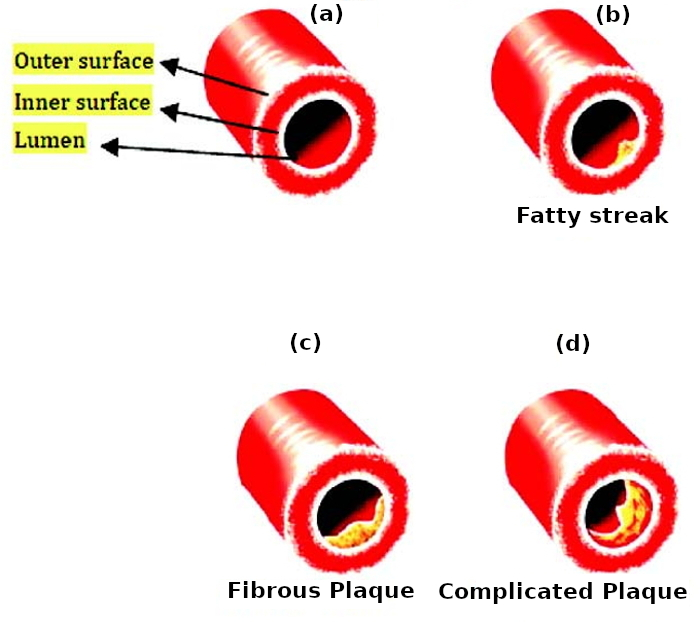
\includegraphics[scale=2.4]{images/038.jpg}
\vskip-.5cm
\end{figure}

\noindent\textbf{What triggers DKA?}

\vskip 5pt

DKA is usually precipitated by some kind of stress on human body such as an infection. The stress causes an increase in the energy\break requirement of the body, thus causing the body to burn fat to provide this extra energy requirement.

\noindent\textbf{Treating DKA}

Treatment involves immediate admission to the hospital, gene\-rous intravenous fluids, insulin drip, and correction of electrolyte abnorma\-lities.

\noindent\textbf{A special note for parents and teachers}

Since DKA is more common with type 1 diabetes, which is the most common type of diabetes seen in children, it is important for the adults (teachers or parents) to be aware of this condition, and its symptoms. It is unlikely that the kids will be able to identify their symptoms. If you see a child who is appearing listless or lethargic, seek immediate medical attention. As explained above, a delay in treatment can lead to death of the young one!

\noindent\textbf{Hyperosmolar Hyperglycemic State (HHS)\index{Hyperosmolar Hyperglycemic State}}

This is the second acute complication that can result from severe hyperglycemia. Unlike DKA, this condition is usually seen in adults. These patients usually have a small amount of insulin. This small\break quantity of insulin is enough to prevent development of ketone acids in the body, but not enough to prevent massive hyperglycemia.

\noindent A few other differences seen in HHS compared to DKA are:

\vspace{-\topsep}
\begin{enumerate}[•]
\itemsep=0pt
\item The blood sugar levels are usually higher. In fact they are as high as 1500 mg/dL. With DKA it is usually \textless 800 mg/dL.
\item The symptoms develop more slowly compared to DKA, taking several days.
\item Neurological complications such as stroke, coma etc are more\break common than in DKA.
\end{enumerate}
\vspace{-\topsep}

This condition is as deadly as DKA, and thus requires prompt\break medical care.

\vskip 4pt
\noindent{\textbf{Hypoglycemia\index{Hypoglycemia}}}
\vskip 4pt

This is the third acute or sudden complication that can develop in diabetics. In contrast to DKA and HHS, where the blood sugar levels are sky high, in hypoglycemia blood sugar levels hit rock bottom. Unlike DKA and HHS, which are a consequence of under treatment or lack of treatment of diabetes, hypoglycemia in diabetics is a consequence of over treatment of diabetes with medications and/or insulin.

Usually hypoglycemia is defined as a blood sugar level below 50 mg/dL. It is lethal if left untreated. Hence it is imperative that both the patients and the doctors treating the patients be well versed with this condition.

Hypoglycemia occurs frequently in many diabetics. In fact, it is an inseparable part of every diabetic’s life. Almost every single diabetic would have experienced this condition at one time or the other. After their first experience they are able to quickly identify its symptoms when it happens again.

\textcolor{blue}{\textit{Every doctor treating a diabetic should educate the patient about hypoglycemia and its management.}}

So what causes this condition? Is it a side effect of medications taken for diabetes? Is it a consequence of higher than required medication dose? Is it a result of improper nutrition? The answer is yes, to all the above!

\noindent\textbf{Symptoms of hypoglycemia}

Hypoglycemia mainly affects the nerves. This is because nerve cells (or neurons) rely solely on glucose as a source of energy.

\noindent The symptoms can be classified into tow categories.

\vspace{-\topsep}
\begin{enumerate}[a)]
\itemsep=0pt
\item \textbf{Symptoms due to dysfunction of the autonomic (independent) nervous system}

The autonomic nervous system controls the involuntary functions in the body, such as the beating of the heart, sweating etc.\break Hypoglycemia can cause a rapid heartbeat (palpitations), profuse sweating, shaking, nervousness or anxiety, tingling sensation,\break hunger etc. These symptoms and signs should sound the warning bell to the patient to quickly consume some sugar, or sugar contai\-ning substance (candy etc). These symptoms tend to develop when blood sugar level is around 58 mg/dl.
 \item \textbf{Symptoms due to dysfunction of the central nervous system}

These include confusion, lethargy, fatigue, difficulty in thinking and speaking, headaches, blurry vision, seizures (“fits”) etc. These symptoms develop when the blood sugar level is below 50 mg/dL (lower than levels needed for autonomic dysfunction).$^{\text{\cite{chap10–key01}}}$
\end{enumerate}
\vspace{-\topsep}

\textcolor{red}{\textit{When the sugar levels are very low, the person may lose consciousness and eventually lapse into a coma, and even death!}}

Sometimes both these categories of symptoms can be seen together. At other times however, symptoms of autonomic dysfunction may not be seen. Instead patients may only have features of central nervous systems dysfunction, namely headache, confusion, agitation, lack of energy or lethargy, memory problems, vision problems etc. In such cases, the first course of action should be to check the blood glucose level, and if hypoglycemia is detected, this should be addressed right away.

Identifying symptoms of hypoglycemia such as headache, dizziness, etc correctly will avoid unnecessary and costly consultations and work–up by various medical specialists such as neurologist, eye specia\-list, ENT (ear, nose and throat) specialists, and even psychiatrists!

There can be several reasons for the lack of signs and symptoms of autonomic nervous system dysfunction in hypoglycemia, as listed below:

\vspace{-\topsep}
\begin{enumerate}[•]
\itemsep=0pt
\item A gradual drop in blood glucose levels
\item Advanced age can blunt the normal response such as sweating, palpi\-tations, shaking, etc to hypoglycemia
\item Taking some medications known as beta blockers for controlling\break blood pressure, can also artificially block certain functions of the\break autonomic nervous system
\end{enumerate}
\vspace{-\topsep}

\noindent This results in a dangerous condition known as “hypoglycemia un-\break awareness”.

\noindent{\textbf{Hypoglycemia unawareness}}

Normally, when blood sugar levels start to drop, the human body tries to counter this by the following mechanisms:
\begin{enumerate}[•]
\itemsep=0pt
\item Decreases insulin secretion, which prevents further drop in blood sugar levels
\item Increases glucagon\index{Glucazon} secretion from the pancreas (glucagon does\break exactly the opposite of insulin, i.e. raises blood sugar level)
\item Increases adrenaline release from the adrenal glands, which causes blood sugar levels to rise
\item Increased adrenaline causes heart palpitations (increased heart rate), sweating, shakiness etc. These serve as early warnings to the human body to consume more glucose (or glucose containing substance) to make sure blood glucose level does not fall further.
\end{enumerate}

Remember that when there is autonomic dysfunction, as seen\break in hypoglycemia unawareness, none of the above compensatory\break mecha\-nisms work. \textcolor{red}{\textit{Hence the patient is completely unaware of the\break dangerous situation developing inside his/her body, and does nothing to help himself/herself, and can eventually slip into a coma and die!}}

\vskip 6pt

\noindent{\large\textbf{Managing hypoglycemia}}

\noindent\textbf{Prevention}

As the saying goes, “prevention is better than cure” when it comes to hypoglycemia. Identifying common triggers for hypoglycemia and preventing them would be the best management.

\noindent The following simple solutions go a long way in this regard:

\vspace{-\topsep}
\begin{enumerate}[•]
\itemsep=0pt
\item Timely and adequate meals and medications: Eat 4 times a day—breakfast, lunch, evening snack and dinner, and take medications as prescribed by your doctor.
 \item If you anticipate doing extra work on any particular day, then you may need to increase your calorie intake. Since you will burn more calories for doing the extra work, you will be at risk for hypoglycemia.
 \item Do not drink alcohol on an empty stomach. Alcohol causes insulin release in your body, and if you do not eat adequately, you are at risk for hypoglycemia.
 \item Talk to your family member, co–workers, classmates about hypoglycemia.They should also be aware of its symptoms and signs, and how they can help you if you were to develop hypoglycemia.
 \item Check your blood glucose levels at different times of the day on\break diffe\-rent days. For example if you check the blood sugar level in\break the morning today, check it in the afternoon tomorrow, and in the eve\-ning the day after tomorrow, and before going to bed on another day. This will give you an idea about your risk of having hypogly\-cemia at a particular time of the day or night. You may see one of the following patterns:
 \begin{enumerate}[o]
\itemsep=0pt
 \item If you notice that your blood sugar in the afternoon is low, then you may have to reduce your dose of short–acting insulin in the morning.
 \item If you notice your evening blood sugar level to be low, then\break the long–acting dose of insulin in the morning may need to be\break decreased. If your blood sugar levels are low at several times\break during day and night, then your medications may have to be\break stopped or their dosage decreased across the board.
\end{enumerate}
\end{enumerate}

\textcolor{red}{\textit{BUT PLEASE DO NOT CHANGE YOUR DOSAGE WITHOUT CONSULTING YOUR PHYSICIAN!}}

\noindent\textbf{What if prevention fails?}

Life is never perfect, and you may still end up having hypoglycemia despite all the above measures. Two actions on your part may end up saving your life in this situation:

\vspace{-\topsep}
\begin{enumerate}
\itemsep=0pt
\item Keeping an emergency source of glucose in your pocket or purse at all times. This could be a candy, chocolate, sugar cubes or anything that is rich in sugar. Put this in your mouth, as soon as you experience the warning signs or symptoms of hypoglycemia.
\item Always carrying a card in your pocket or purse that identifies you as a diabetic. In this card you should also include information about your diabetes medications, and your doctor’s name. In case you are unconscious or in a coma due to hypoglycemia, this information will be invaluable for anyone who comes to your aid.
\end{enumerate}

\noindent\textbf{Responsibility of family members / others}

There are two scenarios in which a family member or any member of the general public plays a vital role in case hypoglycemia develops in a diabetic patient:

\vspace{-\topsep}
\begin{enumerate}
\itemsep=0pt
\item When the person with diabetes is acting strange, i.e. confused, agitated, sweaty, shaking, then immediately provide them some glucose in the form of sugar, candy, chocolate, glucose water, juice, a teaspoon of honey etc.
\item If you see a person with diabetes lying unconscious, imme\-diately obtain medical help. This person may need intravenous (IV)\break glucose solutions to reverse this unconscious state/coma.
\end{enumerate}
\vspace{-\topsep}

\textcolor{blue}{\textit{Do not worry about giving excess glucose in this emergency. Remember that hypoglycemia can sink a person into a coma much faster than hyperglycemic states such as DKA and HHS.}}

\noindent\textbf{The complexity of identifying hypoglycemia}

While the symptoms and signs of hypoglycemia may be quite\break obvious in general, conclusively identifying low blood glucose levels may be difficult for several reasons listed below:

\vspace{-\topsep}
\begin{enumerate}[•]
\itemsep=0pt
\item As soon as the blood glucose level drops, the human body responds to this by decreasing insulin secretion, increasing glucagon\index{Glucazon} secretion, and increasing adrenaline release. This results in blood glucose levels returning to normal or even high levels rapidly.
\item An alert and well–informed patient may have consumed a high\break calorie snack (candy etc) before coming to the doctor’s office, and this will cause the blood sugar level to rise quickly.
\item Many patients and doctors mistakenly check urine sugar levels after an episode of suspected hypoglycemia. But urine levels do not reflect the current situation. Rather it is a reflection of the blood sugar level many hours ago.
\end{enumerate}

But why do we care about correctly identifying low blood sugar levels when symptoms or signs of hypoglycemia occur? This is because both patients and doctors erroneously think that the symptoms were because of high blood sugar levels, and keep on increasing the dose of diabetes medications. Obviously, this is not only wrong, but also dangerous!

So what is the solution? The only answer is to check the blood sugar at the time symptoms and signs are happening, provided there is time to do this. For this to happen the patients will need to have a blood glucose meter with them. But please remember that the first priority in this situation is still to make sure the patient gets a quick source of glucose like sugar, chocolate etc to prevent a coma.

\begin{thebibliography}{99}
\bibitem{chap10–key01} Mitrakou A, Ryan C, Veneman T, Mokan M, et al. Hierarchy of glycemic thresholds for counter–regulatory hormone secretion, symptoms, and cerebral dysfunction. Am J Physiol. 1991; 260(1): E67–74.
 \end{thebibliography}


\chapter{Chronic complications of diabetes}\label{chap11}

\vspace{-\topsep}
\centerline{\Large{\textbf{(The ten diseases caused by diabetes)}}}

\vskip 8pt
Chronic complications are the major burden of diabetes. They weave a web of darkness in the patient’s life.

Diabetes is a disease that can affect any part of the human\break body. Details of each of these complications are beyond the scope of\break this book. Hence, the most important are described in the rest of\break the chapters. These complications are listed below in the order of\break importance and/or magnitude:

\vspace{-\topsep}
\begin{enumerate}
\itemsep=0pt
\item Cardiovascular disease
\item Hypertension and lipid (cholesterol) abnormalities
\item Kidney disease
\item Eye complications
\item Foot diseases
\item Neurologic (nerve) complications
\item Sexual dysfunction
\item Skin diseases and dental complications
\item Joint complications
\item Gastrointestinal complications
\end{enumerate}
\vspace{-\topsep}

\noindent\textbf{How can one disease affect the entire body and cause so many\break complications?}

The answer to this question lies in the fact that diabetes affects the vast network of blood vessels in the human body. The blood vessels are literally the lifeblood of the body, supplying oxygen and nutrients essential for the survival of each and every cell in the human body.

\vskip 3pt
\noindent\textbf{How does diabetes affect the blood vessels?}
\vskip 3pt

\noindent\textbf{The role of Advanced Glycation End Products (AGEs)}

Advanced glycation end products (AGEs) form when glucose in\break the blood is higher than normal. This excess glucose combines with\break proteins and lipids (fat molecules) in the blood. In the early stages, this combination is reversible, provided the glucose level comes back\break to normal. But when the sugar levels in the blood remain high over\break prolonged periods, this binding becomes irreversible. These AGEs\break cause the following adverse effects:

\vspace{-\topsep}
\begin{enumerate}[•]
\itemsep=0pt
\item AGEs accumulate in the walls of the blood vessels, which in turn\break causes the walls to become stiff and lose their elasticity. The same changes are caused by smoking cigarettes!
\item They accumulate in the kidneys and damage the filters. This causes protein to leak into the urine through the damaged kidney filters.
\item They increase cholesterol deposition in the blood vessels, which\break causes plaques. This can lead to heart attacks and strokes.
\end{enumerate}
\vspace{-\topsep}

In fact, research is currently underway to make anti–AGE drugs to combat these effects. \textcolor{red}{\textit{But it is deeply disturbing to note that AGEs are being used as food additives in certain foods, especially in the United States!}}$^{\text{\cite{chap11–key01}}}$$^,$$^{\text{\cite{chap11–key02}}}$

\vskip 5pt
\noindent\textbf{Why do some diabetics develop complications sooner than others?}
\vskip 3pt

A common question I am asked in my clinical practice is “why is it that I have all these complications from diabetes, while others with diabetes for 10 or 15 years more than me, are free of all complications?”

The answer to this questions lies partly in the genetic predis-\break position. Some people are genetically predisposed to develop vascular\break complications such as heart disease, kidney disease, eye (retinal)\break disease, much more than others. Diabetes serves as a catalyst and\break accelerates this process, whereby, they tend to develop these\break conditions much sooner.

Secondly, it is now well known that vascular damage starts\break even before the diagnosis of diabetes. During the phases of impaired\break fasting glucose and impaired glucose tolerance there is ongoing\break vascular damage. As has been previously explained, some unfortunate genetically predisposed individuals develop the ‘pre–diabetes stage’ sooner, and hence vascular damage starts earlier in these individuals.

In conclusion, some individuals are genetically at higher risk\break not only to develop diabetes, but also to develop vascular compli-\break cations. Consequently, they manifest complications many decades\break earlier than others. This is precisely the reason why frequent\break screenings and early diagnosis in genetically predisposed individuals is so crucial. With early diagnosis, measures can be taken to slow or prevent these complications from happening.

Now, we shall proceed to discuss each of the ten disease states\break caused by diabetes.

\begin{thebibliography}{99}
\bibitem{chap11–key01} Peppa M, Uribarri J, \& Vlassara J. Glucose, glycation end products, and diabetes complications: What is new and what works. Clinical Diabetes 2003; 21(4): 186–87.
\bibitem{chap11–key02} Goldin A, Beckman JA, Schmidt AM, \& Creager MA. Advanced\break glycation end products: Sparking the development of diabetic vascular injury. Circulation 2006; 114(6): 597–605.
\end{thebibliography}


\chapter{Cardiovascular disease and stroke}\label{chap12}

\textit{Cardiovascular disease\index{Cardiovascular disease}} is the number one killer in diabetes. It refers to disease of the blood vessels in the human body. \textcolor{blue}{The total length of all blood vessels in the human body is approximately 60,000 miles, and diabetes can affect every inch of this network!}

The two main cardiovascular diseases are coronary artery disease and stroke. Combined, these two diseases account for 65\% of all deaths in \textcolor{red}{Patients with diabetes have a 4–fold higher risk of developing cardiac disease and stroke when compared to people without diabetes.} (Source: American Heart Association). \textcolor{red}{Indians have a 2–3 times higher risk of death from cardiovascular disease than Caucasians even in the absence of diabetes. So obviously the mortality risk due to cardiovascular disease among Indian diabetics should be higher than 4–fold compared to non–diabetics.}

In this chapter we will focus on cardiac disease first and stroke is explained in the second part of this chapter.

We will discuss how the human heart functions under normal\break conditions, what goes wrong in coronary artery disease, why people with diabetes have such a high risk of coronary artery disease, and what can be done to prevent this mortal threat.

\noindent\textbf{The human heart is a miracle machine}

The human heart has variously been described in literature as\break the abode of the Almighty, a poet’s refuge, lovers’ retreat, etc. This\break incre\-dible muscle mass starts pumping blood while still inside the\break mother’s womb, and beats tirelessly till death!

It is an autonomous organ that dances to its own tune. This tune originates from an electric generator known as the Sino Atrial Node (SA Node). This is the pacemaker of the heart. Electrical impulses\break generated here are spread throughout the heart muscles via a network of fibers known as the Purkinje fibers. This is similar to trans\-mission lines carrying electricity produced in power plants. This electri\-city stimulates the heart muscle to beat approximately 72 times per minute. With each beat of the heart, about 60 ml of blood is pumped out into the body.

\begin{figure}[h]
\centering
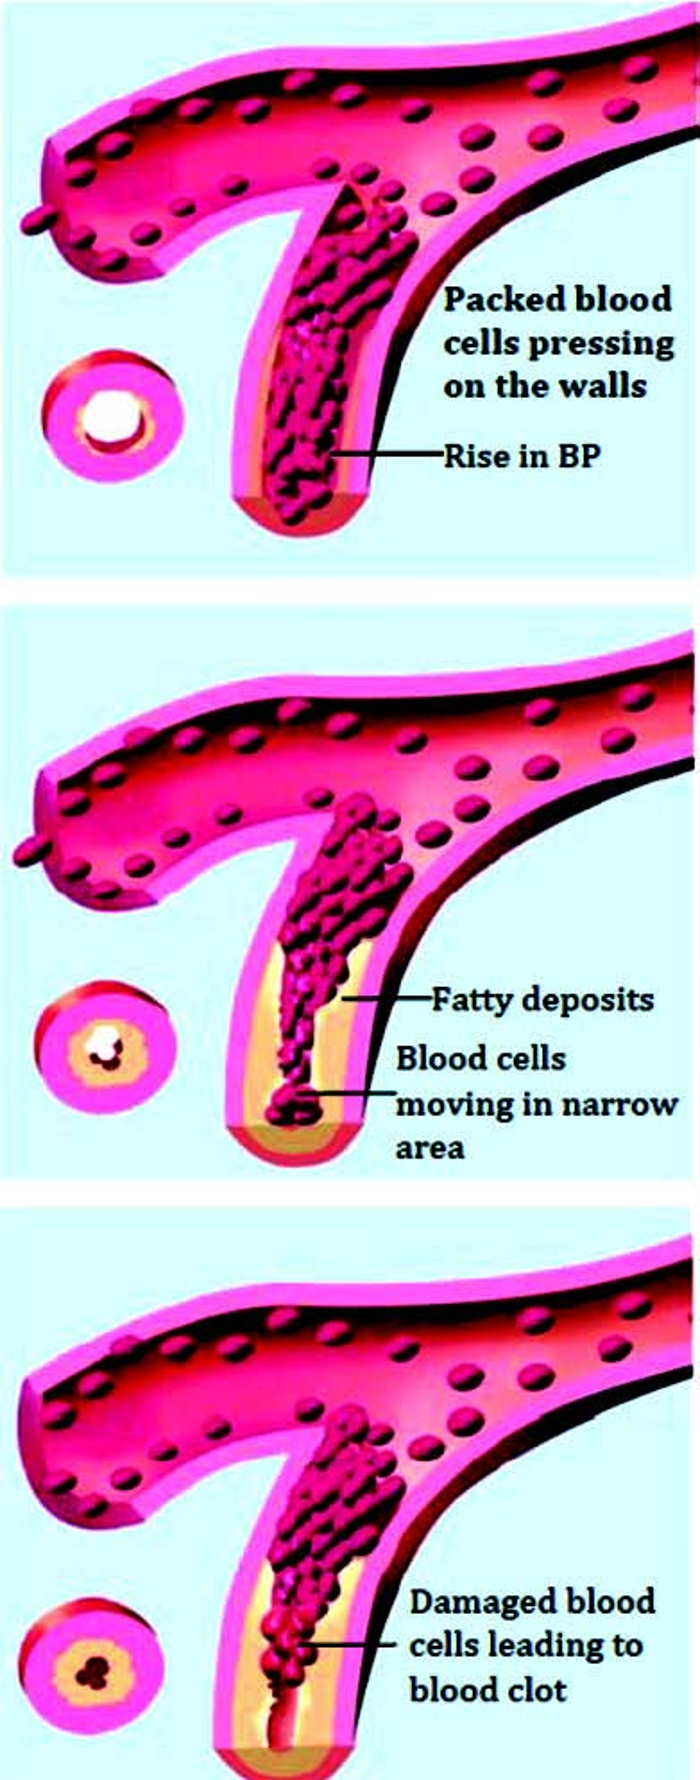
\includegraphics[scale=2.4]{images/039.jpg}\\
\textbf{\textit{Apperance of a normal heart}}
\vskip-.3cm
\end{figure}

Though the four heart chambers are constantly bathed in blood, the heart cannot use this blood for its own nourishment. Instead, it has its own blood supply through the coronary arteries. “Coronary” by definition means, “crown”. The coronary arteries sit atop the heart like a crown, and hence the name. Abnormalities of these coronary arteries cause coronary artery disease, which is the number one cause of death worldwide, and especially so among diabetics.

\begin{figure}[h]
\centering
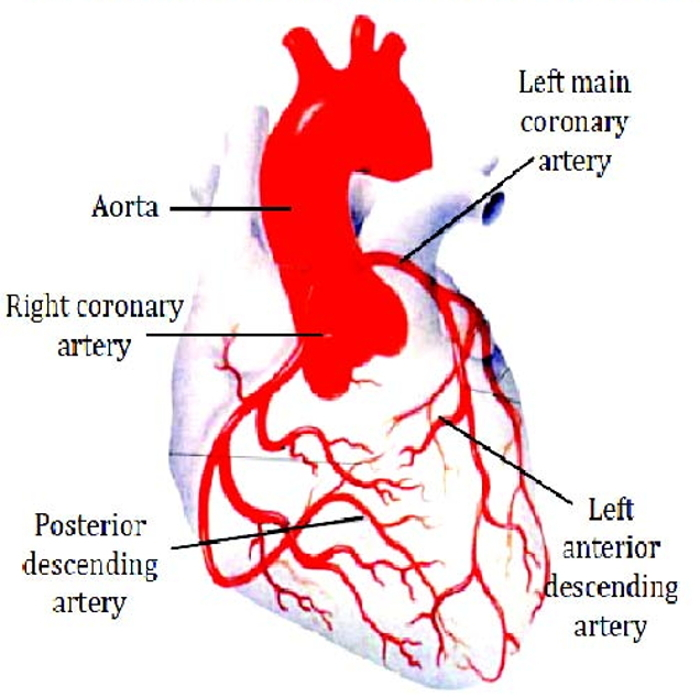
\includegraphics[scale=1.8]{images/040.jpg}\\
\textbf{\textit{Blood Supply to heart Coronary (Crown) Arteries}}
\vskip-.4cm
\end{figure}

\noindent\textbf{What causes coronary artery disease?}

\begin{wrapfigure}{l}{5.8cm}
\centering
\textbf{\textit{Coronary arteries \& plaque formation:}}\\
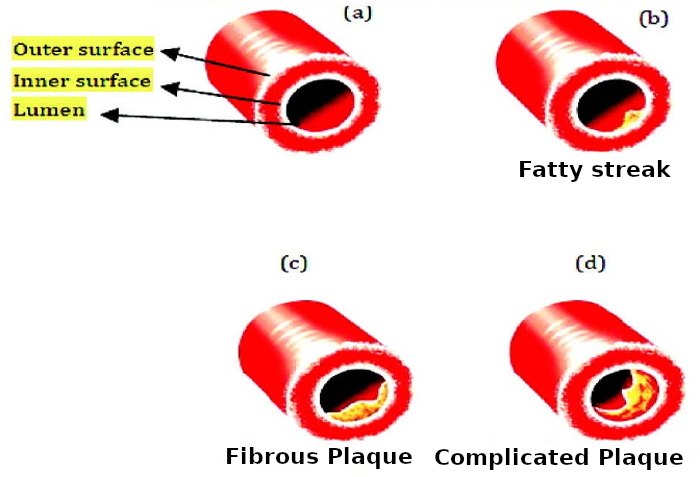
\includegraphics[scale=1.3]{images/041.jpg}
\vskip-.5cm
\end{wrapfigure}

Under normal conditions,\break human blood courses through every blood vessel without\break impediment. The walls of the blood vessels are elastic, and can stretch during periods of increased blood flow, such as during exercise, anxiety, etc.

\begin{wrapfigure}{r}{4cm}
\centering
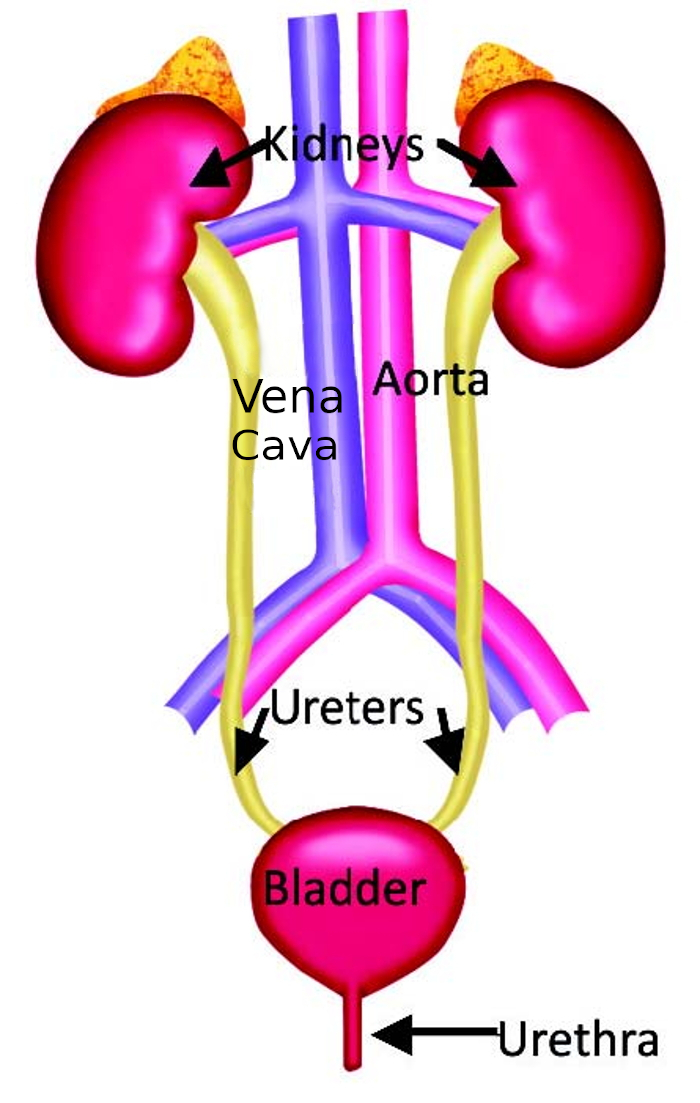
\includegraphics[scale=.9]{images/042.jpg}
\vskip-.4cm
\end{wrapfigure}

Over time however, cho\-lesterol particles flowing\break through human blood start\break depositing on the inner walls of the blood vessels. This cau\-ses choleste\-rol plaque for\-mation in the blood vessels. This plaque progressively increases in size, causing narrowing of the vessel lumen. This narro\-wing prevents the smooth flow of blood through the vessel. Excess pressure is required for the blood to be able to flow through this\break narrowed area. The heart muscle has to pump harder to generate this increased pressure. In addition, this high pressure blood flow gene\-rates shear forces. Shear forces are mighty powerful. In fact, the\break Grand Canyon Arizona, USA, considered to be one of the seven\break natural wonders of the world is a result of shear forces from the flow of the mighty Colorado river ! The cholesterol plaque in the blood vessel is no match for the shear forces of flowing blood and the may suddenly rupture at the surface.

\noindent This may result in two potential outcomes:

\begin{enumerate}
\itemsep=0pt
\item A broken fragment of the choleste\-rol plaque may flow through the blood stream and get stuck in a smaller blood vessel, and block this blood vessel. The part of the heart that depends on this blocked vessel for its blood supply, will be starved of nutrients and asphyxiated of oxygen, and will die.
\item The site of the ruptured cholesterol plaque attracts the cells in the blood. These cells try to plug this break in the surface and form a blood clot. This is the same process that\break happens when we have a cut or nick on our skin. This blood clot can\break completely occlude the lumen, and completely cut off blood supply to the heart muscle supplied by this vessel.
\end{enumerate}

\clearpage
These two scenarios are nothing but the dreaded “heart attack” that can extinguish life in a matter of seconds!

But what if the cholesterol plaque does not rupture as described above. It can still cause damage by impeding blood flow to the heart muscle due to the narrowing it causes in the vessel lumen. Just like a plant deprived of water, this heart muscle deprived of adequate blood withers away and can lead to two outcomes:

\vspace{-\topsep}
\begin{enumerate}
\itemsep=0pt
\item A condition known as “heart failure” wherein the weakened\break heart muscle struggles to pump blood
\item Angina or chest pain, which is caused by the inability to increase blood flow through the narrowed artery during times of increa\-sed demand for blood flow such as exercise and mental stress.
\end{enumerate}
\vspace{-\topsep}

\noindent{\textbf{Heart disease in diabetes: silent but deadly!}}

Diabetics may be hale and hearty before going to bed at night, and may never wake up. They may be walking around going about their routine, and unexpectedly drop dead!

They experience what is known as “silent MI (myocardial\break ischemia)”. Up to 28 to 37\% of patients with diabetes experience this kind of a heart attack.$^{\text{\cite{chap12–key01}}}$

In general heart attacks are felt as a crushing pain in the chest. But diabetics may not experience any pain at all! Why is this so? Due to the decline in blood supply to the nerves in diabetes, the neural network between the heart and brain becomes dysfunctional. Thus the brain does not hear the cry of a dying heart. Instead the person may feel vague symptoms such as dizziness (due to a drop in blood pressure), sweating, etc, or no symptoms at all!

In order to avoid this frightening prospect, it is important to\break identi\-fy patients at risk for this, and to take preventive measures.

\noindent{\textbf{Why are diabetics at increased risk for coronary artery disease?}}

As previously mentioned, diabetics are at 4 times higher risk for cardiac disease. This is because people with diabetes usually have some or all of the following conditions that increase their risk for coronary artery disease.

\vspace{-\topsep}
\begin{enumerate}[•]
\itemsep=0pt
\item Insulin resistance
\item Hypertension
\item Abnormal cholesterol and high triglycerides
\item Obesity
\item Lack of physical activity
\item Smoking
\end{enumerate}
\vspace{-\topsep}

Further, diabetes increases the severity of each of the above\break conditions.

\vskip 6pt
\noindent\textbf{Prevention of coronary artery disease in diabetes}
\vskip 3pt

It would be wrong to assume that coronary artery disease is a\break foregone conclusion in diabetes, and to lose hope and simply wait for the inevitable.

With appropriate care coronary artery disease can be prevented. The recommended care is well summarized by the National Diabetes Education Program (NDEP), which is the leading federal government source of information about diabetes prevention and control. It is\break spo\-nsored by the National Institutes of Health (NIH) and Center for Disease Control (CDC),USA.

\noindent The mantra proposed by NDEP is \textcolor{blue}{“Control the ABCs of diabetes”.}

\vspace{-\topsep}
\begin{enumerate}[\ding{118}]
\itemsep=0pt
\item A is for A1c in the HBA1c. This gives the 3 month average of\break blood sugar levels. As mentioned in the previous chapter, high\break blood sugar levels lead to formation of AGEs (Advanced Glycation End Products) that accumulate in the walls of the coronary artery, and render the walls hard and inelastic. This results in increased blood pressure. Ideally the HBA1c level should be below 7.
\item B is for Blood pressure. Approximately 60\% of diabetics will have high blood pressure. By maintaining the blood pressure below\break 130/80 mm Hg, the risk of coronary artery disease is reduced.
\item C is for Cholesterol. A characteristic pattern of abnormal lipids is seen in patients with diabetes, and is called “diabetic dyslipidemia”. These patients have high LDL cholesterol (the ‘bad cholesterol’), low HDL cholesterol (the ‘good cholesterol’) and high triglycerides. This triad is often seen in premature coronary artery disease. Prevention of this condition is key to preventing coronary artery disease. This is discussed in more detail in the next chapter.
\end{enumerate}

\begin{figure}[h]
\centering
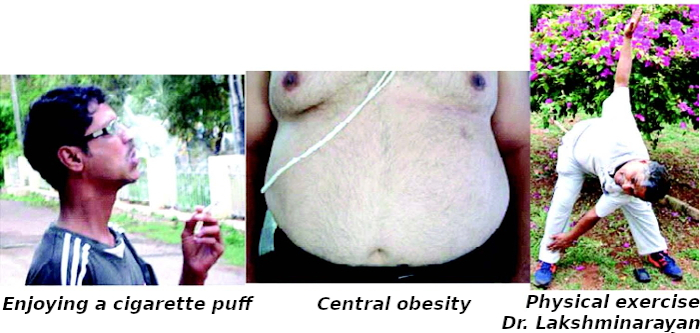
\includegraphics[scale=2.4]{images/043.jpg}
\vskip-.1cm
\end{figure}

In addition to the ABCs, smoking cessation, tackling obesity,\break and exercise are vital to preventing coronary artery disease.

\noindent{\textbf{Screening for coronary artery disease in diabetes}}

Despite the best preventive efforts, coronary artery disease may still occur in diabetes. Further, it may progress very silently without causing any of the usual symptoms of coronary artery disease such as chest pain. For this reason, \textcolor{blue}{it is important to screen patients with dia\-betes for coronary heart disease, even if they are without any\break complaints such as chest pain with exertion etc.} The following simple and safe tests are some of the ways to screen for presence of coronary artery disease:

\clearpage
\begin{enumerate}
\itemsep=0pt
\item \textbf{\textit{ECG or electrocardiography\index{ECG or Electrocardiography}:}} This is a record of the electrical\break activity of the heart. Abnormalities in this electrical pattern can alert the doctor to abnormalities of the heart muscles that may be seen with coronary artery disease.
\item \textbf{\textit{Echocardiography:}} This is an ultrasound examination of the\break heart. This is the same technique used to examine the growing fetus in a mother’s womb! In this test, the structure of the heart walls, and heart valves can be assessed. In addition, the beating of the heart muscles can be seen. The flow of blood through the four different chambers of the heart and into the major arteries emanating from the heart (the pulmonary artery and aorta) can also be examined. Abnormalities in any of these parameters may identify an ailing heart or a heart at risk for complications due to coronary artery disease.
\item \textbf{\textit{Stress test (Treadmill test)\index{Stress test (treadmill test)}:}} In this test, the heart function is\break assessed (either by examining the electrical activity of the heart i.e. ECG, or by ultrasound examination i.e. echocardiography), when the heart is under stress by having the person walk on\break a treadmill. If the person is unable to walk (due to knee joint\break pro\-blems etc), a medication is injected into the blood that causes the heart to beat faster than normal (called ‘dobutamine stress test’). Often, the ECG or echocardiogram may be normal when the person is at rest. But when the heart is beating fast, it\break requires more blood supply. If there is narrowing in any of the supply arteries (i.e. coronary artery disease), then the muscle that is supplied by such a diseased artery will not contract normally and neither will it generate normal electrical impulses. This distress call of the heart muscle is identified by a stress test.
\item \textbf{\textit{Nuclear scans\index{Nuclear scans}:}} In this test, a chemical such as technetium is\break injected into the blood. This chemical flows through the blood and tends to accumulate in the heart cells. Later a special\break camera (gamma camera) is used to image the heart. This\break camera is specially designed to detect technetium. The images of the heart are analyzed. If there are areas of the heart that have very little or no technetium, this means that this area of the heart is either not getting any blood or is getting very little due to coronary artery disease.
\end{enumerate}

\vskip-.3cm
Once coronary artery disease is identified by any of the 4 methods described above, several measures of treatment can be initiated.

\noindent{\textbf{\textit{STROKE\index{Stroke}}}}

Stroke is a dreaded and devastating event that can kill within\break minutes, or worse, paralyze for life. Stroke is to the brain what a heart attack is to the heart. In both conditions there is a sudden stoppage of blood flow. The brain cells are exquisitely sensitive and need a constant supply of glucose and oxygen in order to survive. If deprived of blood flow for as little as 1 minute the cells start to shut down, and are dead by 3 hours!

\noindent There are two main causes for stroke:

\vspace{-\topsep}
\begin{enumerate}
\itemsep=0pt
\item The most common cause is a blood clot that blocks a blood\break vessel supplying the brain. This is called an ischemic or embolic stroke. Ischemic stroke accounts for 85\% of all strokes. This type of stroke is often seen with diabetes.
\item A less common cause is due to a blood vessel that bursts open due to very high pressure inside it. This is called a \textit{“hemorrhagic stroke”\index{Haemorrhagic stroke}}, since there is hemorrhage or bleeding from the burst\break vessel. This type of stroke is usually a consequence of high blood pressure.
\end{enumerate}
\vspace{-\topsep}

\noindent\textbf{How common is stroke in diabetics?}

Unfortunately it is very common. Diabetics have a 2 to 4 times higher risk of developing an ischemic stroke compared to people who do not have diabetes.

\noindent\textbf{Why is there an increased risk of stroke among diabetics?}

The major risk factors for a stroke are hypertension and high chole\-sterol. Diabetics have a 3 times higher risk of developing hypertension than people without diabetes.$^{\text{\cite{chap12–key02}}}$ As many as 2 out of 3 adults with dia\-betes have high blood pressure according to the American Diabetes\break Association.

Diabetics are also more prone to have unhealthy cholesterol\break patterns, and this is termed \textit{“diabetic dysplipidemia”\index{Diabetic dysplipidemia}}, and is explained in more detail in chapter \ref{chap13B}.

In addition to these two major reasons, there are other risk factors for stroke as listed below:

\vspace{-\topsep}
\begin{enumerate}[•]
\itemsep=0pt
\item Age \textgreater  65 years
\item A history of mini stroke or stroke in the past
\item A family history of stroke
\item Heart disease
\item Obesity and being overweight
\item Smoking doubles the risk of stroke
\end{enumerate}

\noindent\textbf{Is stroke preventable?}
\vskip 6pt

Absolutely! Since we know the risk factors for a stroke, modi\-fying these risks can prevent a stroke. According to the National Stroke\break Association of USA, up to 80\% of strokes are preventable.

\noindent The following measures are recommended to prevent a stroke:

\vspace{-\topsep}
\begin{enumerate}[•]
\itemsep=0pt
\item Many people with high blood pressure may not be aware that they have hypertension, and tragically a stroke may be the first sign.\break Hence regular screening for high blood pressure is recommended.
\item If diagnosed to have high blood pressure, adequate blood pressure control prevents risk of stroke.
\item Have your cholesterol checked and take measures to keep it under control.
\item If you smoke, quit!.
\item Do not consume excess alcohol.
\item Exercise regularly.
\item Keep your body weight under control.
\item Have a routine cardiac check up. Irregular heart rhythm (called \textit{atrial fibrillation\index{Atrial fibrillation}}) is a major risk factor for stroke. Taking a blood thinner such as aspirin or warfarin can significantly reduce this risk.
\end{enumerate}
\vspace{-\topsep}

\vskip 4pt
\noindent\textbf{How do I know if I am having a stroke?}
\vskip 4pt

Despite our best efforts, a stroke may occur. Early diagnosis and treatment is the best bet to stay alive and avoid paralysis. The faster the blood supply to the brain is restored, the fewer brain cells die. You can play a major role in this situation by identifying the symptoms and signs of stroke. These are listed below:

\vspace{-\topsep}
\begin{enumerate}[•]
\itemsep=0pt
\item Numbness or weakness on one side of the face, arms or legs
\item Loss of vision or dimming of vision, especially in one eye
\item Loss of speech or slurring of words
\item Dizziness without an alternative explanation like low blood pressure due to medications, or low blood sugar
\item Sudden severe headache
\end{enumerate}
\vspace{-\topsep}

If any of these happen to you, call an ambulance right away, and head to a hospital that is well versed in treating stroke patients. If you make in time, then a medicine (popularly called “clot busters’) can be injected into your veins that can dissolve the blood clot blocking the blood supply to your brain to prevent death and disability. But the\break doctors will first make sure that there is no bleeding in your brain by doing a CT scan of your head, because in the rare case that you have a hemorrhagic stroke, then clot busting drugs will only make the\break bleeding worse.

\clearpage

\begin{thebibliography}{99}
\bibitem{chap12–key01} Kwong RY et al. Circulation 2008; 118: 1011–20; Nesto RW et al. Am Heart J 1990;120: 1073–77
\bibitem{chap12–key02} Sowers JR et al. Hypertension 2001; 37: 1053–59
\end{thebibliography}


\newpage
 
\renewcommand{\thechapter}{\arabic{chapter}A}
\chapter{Hypertension and diabetes}\label{chap13A}

\textit{Hypertension\index{Hypertension}} or high blood pressure is commonly seen in approximately 60\% of diabetics.

Blood pressure is nothing but the force exerted by the flow of blood inside our blood vessels. When blood flows with excess force, it exerts increased pressure or tension on the walls of the blood vessels, and it is termed ‘high blood pressure’ or ‘hypertension’.

The pressure in our blood vessels can be measured easily, and it is expressed as two numbers. Normal blood pressure is less than 120/80 millimeters of mercury (mm Hg).

The top number or numerator here is termed systolic blood pre\-ssure. This is the pressure in our blood vessels when our heart squeezes and pushes blood out into the blood vessels to reach the rest of the body. The bottom number or denominator is termed diastolic blood pre\-ssure, and it is the pressure in the blood vessels when the heart is in its relaxed state, when blood is returning to the heart from the rest of the body.

Hypertension is diagnosed when the blood pressure exceeds 140/90 mm Hg on more than two different occasions.

\vskip 10pt
\noindent\textbf{What causes high blood pressure?}

In 95\% of patients, no clear cause can be identified for high blood pressure, and this is termed essential hypertension.

In the remaining 5\% kidney problems, adrenal gland tumors\break (which sits on top of the kidneys, and secretes adrenaline), certain medications (such as birth control pills, etc) can cause high blood\break pressure.

\vskip 10pt
\noindent\textbf{What are the risk factors for developing high blood pressure?}

\noindent Several factors contribute for hypertension exist, and they include:
\begin{enumerate}[•]
\itemsep=0pt
\item Age
\item Family history of high blood pressure
\item Diabetes
\item Obesity and being overweight
\item Physical inactivity
\item Tobacco use
\item Excess salt intake in diet
\item Excess alcohol consumption
\item Stress
\item Certain chronic disease such as kidney disease, high cholesterol\break levels, etc.
\end{enumerate}

As you may notice several factors mentioned above are also risk factors for development of diabetes, namely – age, obesity, inactivity, stress.

\textcolor{red}{\textit{In fact diabetics have a 3–times higher risk to develop hypertension than people without diabetes.}}$^{\text{\cite{chap13–A–key01}}}$ \textcolor{red}{\textit{As many as 2 out of 3 adults with diabetes have high blood pressure according to the American Diabetes Association.}}

\vskip 8pt
\noindent\textbf{Consequences of high blood pressure in diabetes}

Constant increased pressure in the blood vessels can result in three outcomes:

\vspace{-\topsep}
\begin{enumerate}
\itemsep=0pt
\item Increased workload for the human heart. The poor heart has\break to pump against this increased pressure with every beat. This\break ultimately takes a toll on the heart muscle, which initially\break becomes bulky (called cardiomyopathy), but becomes feeble\break over time. This process can result in fatal conditions such as:
\begin{enumerate}
\itemsep=0pt
 \item Heart attack. Diabetics are at twice the risk of those\break without diabetes for death from cardiac causes.
\item Irregular heart rhythms.
\item Heart failure.
\end{enumerate}
\item Hardening of walls of the arteries. Relentless pressure exerted by blood flow culminates in the loss of the elastic nature of the walls of the blood vessels. The walls thicken, harden and become narrowed. This results in decreased blood flow to vital organs, resulting in:
\begin{enumerate}
\itemsep=0pt
\item Nephropathy or kidney failure
\item Retinopathy or disease of the inner eye resulting in blindness
\item Stroke
\end{enumerate}
\item \textit{Aneurysms\index{Aneurysm}:} This is a life threatening condition. A part of the wall of the artery bulges out due to the unrelenting force of blood flow. This bulge is called an aneurysm. Due to the stretch caused by the bulge, this part of the vessel wall is weak, and is prone to rupture or bursting open. Such a bulge can form anywhere in the body. If it forms in the brain, aorta (the largest artery in the body), or other vital areas, then its rupture can cause instantaneous death!
\end{enumerate}
\vspace{-\topsep}

\textcolor{red}{\textit{All the above complications are both more common in diabetics (by\break 2–3 times compared to the general population) and also occur much earlier in life.}}$^{\text{\cite{chap13–A–key02}}}$


\noindent\textbf{Management of high blood pressure in diabetes}

As with any medical condition, the first and foremost step in\break management is diagnosis.

\textcolor{red}{\textit{Hypertension is a silent assassin that usually does not cause\break symptoms until it is too late!}} So please do not make the grave mistake of wai\-ting for symptoms! Many people associate high blood pressure with headaches, but the fact is that people with high blood pressure are up to 40\% less likely to have headaches than those with normal blood pre\-ssure (Source: American Heart Association)!

\vskip 6pt
\textcolor{blue}{\textit{The best way to diagnose high blood pressure is by screening, i.e. checking blood pressure regularly.}}
\vskip 6pt

Once the diagnosis is established, it is crucial to realize that this condition is chronic, and needs chronic management, just like diabetes. Details of management, while beyond the scope of this book, are\break simple and easy to follow, as elucidated in the following recommenda\-tions by the American Heart Association.

\vspace{-\topsep}
\begin{enumerate}
\itemsep=0pt
\item Eat a better diet.
 
The DASH (Dietary Approaches to Stop Hypertension) diet is a\break dietary plan formulated by research conducted at Harvard, Johns Hopkins and Duke Universities in USA. This is widely promoted by the United States Department of Health and Human Services (DHS). This diet is low in salt, sugar and fat, but rich in fruits, vege\-tables, and whole grains. This diet decreased blood pressure by about 11 mg Hg (for example from 140 mm Hg to 130 mm Hg) after just 3 weeks according to one study.$^{\text{\cite{chap13–A–key03}}}$

 In fact following a DASH diet may have the potential to prevent type 2 diabetes.$^{\text{\cite{chap13–A–key04}}}$
\item Enjoy regular physical activity. At least 30 minutes of total exercise time on most days of the week can reduce the blood pressure by 5–10 mm of Hg.
\item Maintain a healthy weight (prevent obesity)
\item Manage stress through yoga, meditation, etc.
\item Avoid smoking
\item Take medicines as advised
\item Limit alcohol intake
\end{enumerate}
\vspace{-\topsep}

You will no doubt notice that all of these recommendations are similar to the recommendations to prevent or treat cardiovascular\break disease discussed in the previous chapter.

The goal of therapy in diabetics is to achieve a blood pressure of less than 130/80 as recommended by the American Diabetes Association.

\noindent\textbf{Special considerations in choosing blood pressure medications\break when treating diabetics:}

Diabetics need special medicines to treat high blood pressure when compared with patients without diabetes. \textcolor{red}{\textit{Some commonly used medicines namely diuretics (“water pill”) and beta blockers can actually worsen diabetes control.}}

It is recommended to use ACE (angiotensin converting enzyme)\break inhibitors (such as enalapril, lisinopril etc) or ARBs (angiotensin\break receptor blockers) such as losartan in diabetes. These drugs have the added advantage of protecting the kidneys in the long run. The other recommended group of medication is calcium channel blockers such as amlodipine.$^{\text{\cite{chap13–A–key05}}}$

\begin{thebibliography}{99}
\bibitem{chap13–A–key01} Sowers JR, Epstein M, \& Frohlich ED. Hypertension 2001; 37(5): 1053–59.
\bibitem{chap13–A–key02} Reboldi G, Fentile G, Manfreda VM, Angeli F, \& Verdecchia P. Tight blood pressure control in diabetes: evidence–based review of treatment targets in patients with diabetes. Curr Cardiolo Rep. 2012; 4(1):89–96.
\bibitem{chap13–A–key03} Moore TJ, Conlin PR, Ard J, \& Svetkey LP. DASH (Dietary Approaches to Stop Hypertension) diet is effective treatment for stage 1 isolated systolic hypertension. Hypertension. 2001; 38(2):155–8.
\bibitem{chap13–A–key04} Liese AD, Nichols M, Sun X, D’Agostino RB JR, \& Haffner\break SM. Adherence to the DASH Diet is universally associated with\break incidence of type 2 diabetes: the insulin resistance atherosclerosis study. 2009; 32(8):1434–6.
\bibitem{chap13–A–key05} Bakris GL, Sowers JR, Giles TD, Black HR, Izzo JL Jr, et al. Treatment of hypertension in patients with diabetes– an update. J Am Soc Hypertens. 2010; 4(2):62–7.
\end{thebibliography}

\newpage
 
\setcounter{chapter}{12}
\renewcommand{\thechapter}{\arabic{chapter}B}
\chapter{Cholesterol and diabetes}\label{chap13B}

\textit{Cholesterol\index{Cholesterol}} is a soft waxy substance present both in blood and inside\break human cells. It is a form of fat. The word cholesterol originates from the Greek words ‘chole’ meaning bile and ‘sterol’ meaning solid. In other words, solidified fat seen in bile juice. The liver secretes bile juice, and the liver is the main source of cholesterol synthesis.

Of all the medical terms, “cholesterol” is one name that evokes\break universal dislike among the general public. It is blamed for heart\break attacks, strokes, high blood pressure, etc. Unfortunately for choleste\-rol, this is all true!

But it would be wrong to blame cholesterol for all our indiscretions. We humans have a tendency to misuse anything and everything God has given us. God gave us a vegetable, and we fry it and douse it with salt and call it potato chips. God gave us fruit, and we drown it in sugar and call it jam. God gave us pure water, and we adulterate it with\break artificial flavors to make colas. The list is endless.

God did not create cholesterol to cause heart attacks. He meant cholesterol to be a vital part of the human cell membrane; to be an\break essential element in the synthesis of sex hormones such as testosterone and estrogen, without which no human can have an offspring; and to offer many other benefits for mankind.

Moreover, not all cholesterol is created equal. The good form of cholesterol, namely HDL cholesterol actually protects against heart\break disease!

The bad cholesterols are the LDL (Low Density Lipoprotein) and triglycerides. They promote heart disease. They tend to stick to the insides of the blood vessels. The body’s immune system tries to scrape these off, but actually converts the fat into a more toxic form. This toxic form of cholesterol now attracts more immune cells, which\break try to destroy it, but some immune cells die in the fight. Hence a\break miniature battlefield is created at this site. The combination of bad chole\-sterol, immune cells and dead cells result in ‘cholesterol plaque’ formation. This plaque progressively increases in size and occludes the blood vessel either partially or completely.

\begin{figure}[h]
\centering
\textbf{\textit{Coronary arteries \& Plaque formation:}}\\
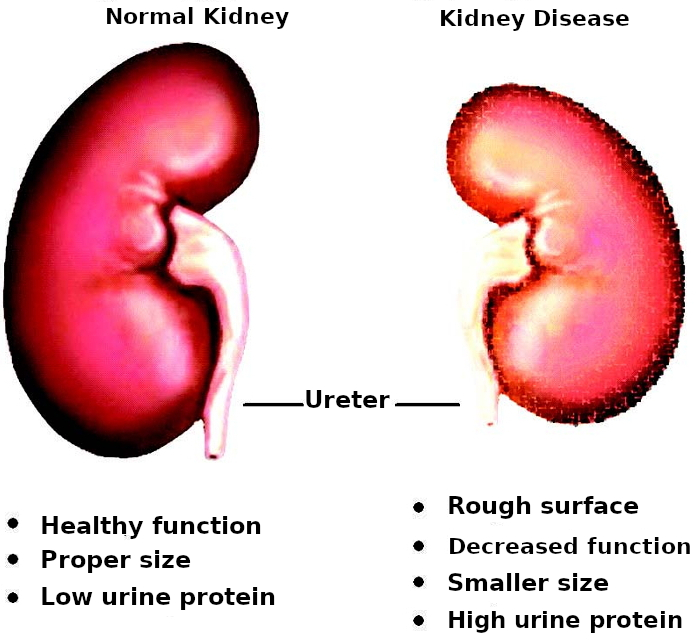
\includegraphics[scale=1.9]{images/044.jpg}
\end{figure}

Unfortunately people with diabetes are prone to having unhealthy cholesterol levels, and hence are at higher risk of cardiac disease. This condition is termed \textit{“diabetic dyslipidemia.”}

\noindent{\textbf{\textit{Diabetic dysplipidemia}}}\index{Diabetic dysplipidemia}

This is a characteristic pattern of cholesterol in people with diabetes, in which the good cholesterol i.e. HDL cholesterol levels are low; bad cholesterol and triglyceride levels are high.

While the exact cause for this pattern is not clear, it is most likely a result of defective insulin action.

\textcolor{red}{\textit{This pattern is not just limited to full–blown diabetes, but is also seen in the ‘prediabetes’ stage! Thus, while the person is blissfully unaware of being at risk for diabetes, the ‘seeds of destruction’ are being sown (cholesterol plaques in the blood vesels).}}

\noindent{\textbf{Managing cholesterol in diabetes}}

The first step in management is diagnosis. \textit{There are no symptoms of high cholesterol, only complications!}

Cholesterol levels are checked by a blood test known as ‘lipid\break panel’. This should be checked after an overnight fast to avoid\break inaccuracies. Recent ADA guidelines recommend after food also.

\noindent{\textbf{Cholesterol targets in diabetes}}

The American Diabetic Association and the American Heart\break Association recommend the following targets to reduce the risk of\break cardiovascular disease and death:

\vspace{-\topsep}
\begin{enumerate}[•]
\itemsep=0pt
\item LDL Cholesterol should be less than 100 mg/dl
\item HDL Cholesterol should be higher than 40 mg/dl for men and\break 50mg/dL for women
\item Triglycerides should be less than 150 mg/dl
\end{enumerate}
\vspace{-\topsep}

\noindent\textbf{How can I achieve these cholesterol goals?}

One should be heartened to know that there is considerable\break overlap among measures aimed to control blood sugar and cholesterol and high blood pressure. In other words you get 3 for the price of 1!

Thus, the recommended measures are largely the same as described in the previous chapters, namely:

\vspace{-\topsep}
\begin{enumerate}
\itemsep=0pt
\item Diet: A DASH (Dietary Approaches to Stop Hypertension)\index{DASH (Dietary Approaches to stop hypertension)} diet is\break helpful to control cholesterol as well. In addition to the DASH diet, it is important to make smart food choices.
\item Enjoy regular physical activity. At least 30 minutes of total\break exercise time on most days of the week.
\item Maintain a healthy weight (prevent obesity)
\item Avoid smoking
\item Avoid excess alcohol
\item Take medicines as advised
\end{enumerate}
\vspace{-\topsep}

\noindent\textbf{Eating smart, the key to eating healthy}

Eating healthy does not have to mean depriving yourself of\break taste buds of any pleasure. ‘Knowledge is power’ when it comes to diet. For example did you know that by avoiding saturated fats (butter,\break animal meats, other milk products, coconut oil, palm oil, etc) and trans fats (hydrogenated oils used in fast food restaurants, frozen pizzas,\break coffee creamers, etc), and instead using mono and polyunsaturated fats (seen in olive oil, sunflower oil, canola oil, nuts, seeds, fish etc), you can\break actually lower your cholesterol level!

Diet in diabetes is discussed in greater detail later in this book.

\newpage
\renewcommand{\thechapter}{\arabic{chapter}}
\chapter{Kidney disease\index{Kidney disease} in diabetes}\label{chap14}

\noindent{\textbf{The human kidneys}}

Our body has 2 kidneys, each about the size of a fist. They are\break located on either side of our spine below the rib cage.

\begin{wrapfigure}{l}{5cm}
\vskip-.5cm
\centering
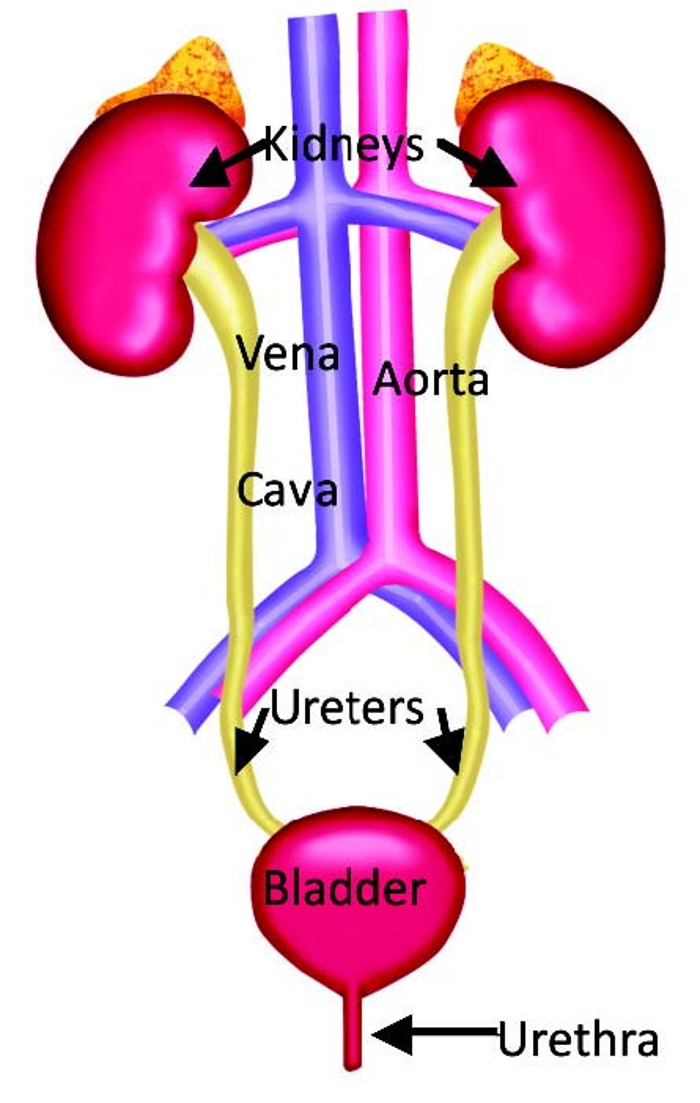
\includegraphics[scale=1.2]{images/045.jpg}
\vskip-.5cm
\end{wrapfigure}

The kidneys are extremely sophisticated machines that perform several vital functions. If you think urine formation is the kidney’s only job, then you don’t know the kidney well enough! It secretes critical hormones that help maintain our blood pressure, notably renin. In addition, it converts vitamin D to its\break active form. Activated vitamin D is important for maintaining our bone strength. Kidneys also secrete a hormone called erythropoietin that is vital in stimulating the bone\break marrow to make red blood cells.

\begin{wrapfigure}{r}{6.4cm}
\centering
\textbf{\textit{Nephron}}\\
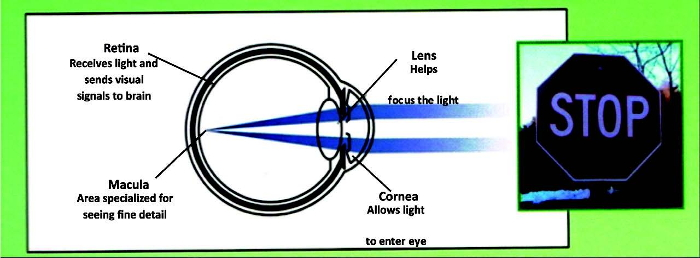
\includegraphics[scale=1.4]{images/046.jpg}
\vskip-.5cm
\end{wrapfigure}

Urine formation in the human body is one of nature’s marvels. It helps excrete toxic byproducts of the various chemical reactions that take place in our body every minute. It also helps maintain the fluid and pH balance in the body.

Urine formation happ\-ens inside tiny units of the kidneys known as neph\-rons. There are approximately 1 million nephrons in each kidney. So each hu\-man body has a total of about two million neph\-rons or filtration units.

Each nephron is composed of a cluster of very tiny blood vessels called capillaries. The walls of these capillaries have tiny pores or holes in them. This capillary cluster is called the glomerulus. The glomerulus acts as a sieve or a filter through which blood is filtered. The pores of this filter are large enough to allow fluids, body salts, glucose and urea (by–product of protein) to leak out, but small enough to prevent proteins in the blood from leaking out. Every minute these nephrons filter out 125 ml of urine, which equates to 7.5 liters every hour and a whopping 180 liters every day!

Can you imagine urinating 180 liters a day? Of course not. Because the nephrons are so sophisticated that they reabsorb 99\% of these 180 liters, to produce only about 2 liters of urine per day. This is possible because surrounding the glomerulus or capillary cluster is a very advanced collection system.

In addition to reabsorbing water, this collecting system will\break reabsorb all the glucose from the filtrate. It will assess how much\break electrolytes (such as sodium, potassium, etc) the body needs, and\break reabsorbs only that much, allowing the rest to flow out in the urine.

In the final stage (called the secretion stage), this collection system will excrete ammonia and by–products of medicines that we use into the urine.

\begin{wrapfigure}{l}{5.9cm}
\centering
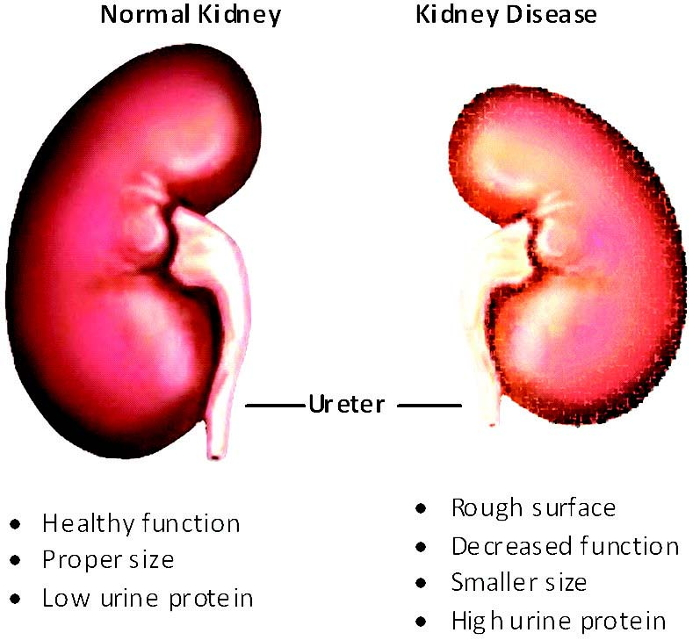
\includegraphics[scale=1.4]{images/047.jpg}
\vskip-.5cm
\end{wrapfigure}

These three stages of\break filtration, reabsorption and\break secretion happen in every\break nephron. So each of 2 million nephrons produces a small quantity of urine. This urine is collected by the kidney and transported to the urinary\break bladder by two tubes known as ureters. Once the urinary bladder fills up, we get the urge to urinate.

Now you know the incredible story behind each drop of urine, which is nothing but finely filtered blood!

\noindent{\textbf{Diabetic kidney disease or diabetic nephropathy}}

Diabetes is the \#1 cause of chronic kidney damage in many\break countries around the world. For example in the US, it accounts for 40\% of all new cases of chronic kidney disease.$^{\text{\cite{chap14–key01}}}$

\begin{wrapfigure}{l}{6cm}
\centering
\textbf{\textit{Diabetes Affects the Kidney}}\\
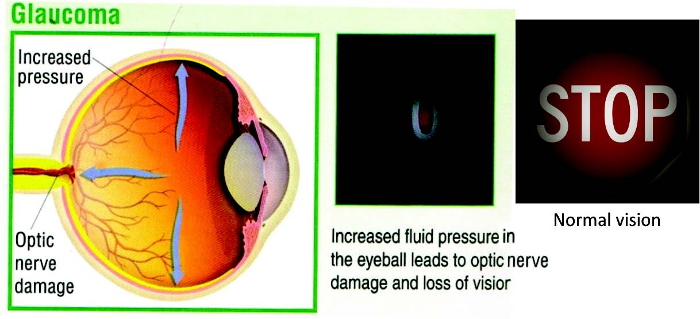
\includegraphics[scale=1.4]{images/048.jpg}
\vskip-.4cm
\end{wrapfigure}

\textcolor{red}{\textit{In the first survey of the causes of chronic kidney di\-seases in India that was published in 2012, diabetes was the main cause accounting for 31\% of cases.}} High blood pressure in comparison accounted for 13\% of cases.\break In fact the combination of diabetes and hypertension is res\-ponsible for more than 2/3 of all cases of chronic kidney\break disease according to the Na\-tio\-nal Kidney Foundation of the United States. According\break to their research, 30\% of\break patients with type 1 diabetes, and up to 40\% of patients with type 2 diabetes will eventually develop diabetic nephropathy.

\textcolor{red}{\textit{You will be not happy to know that diabetics of Indian origin in the UK had a 10–fold higher risk than Caucasians of developing kidney failure requiring dialysis\index{Dialysis}.}}$^{\text{\cite{chap14–key02}}}$ \textcolor{red}{\textit{while Indians living in the Netherlands had a 40–fold higher risk than Caucasians.}}$^{\text{\cite{chap14–key03}}}$

\noindent\textbf{How does diabetes damage the kidneys?}

\noindent Diabetes attacks the kidneys on several fronts:

\vspace{-\topsep}
\begin{enumerate}[\ding{118}]
\itemsep=0pt
\item Primarily it overworks the kidneys. As you know there is excess glucose in the body of diabetics. And whose job is it to remove this excess? The poor kidney’s of course, since urine is the only exit route for this excess sugar. In order to remove this excess sugar, excess filtration has to take place in the nephrons. It is because\break of this excess filtration that people with diabetes have to urinate\break excessively. But the industrious kidneys never complain and go about their extra work quietly. But eventually this workload takes a toll on them and causes damage.
\item Secondly, you would recall that excess glucose forms AGEs or\break Advanced Glycation End products. These AGEs accumulate in the neph\-rons, and in the walls of the blood vessels. This damages the filtration system in the nephrons, which starts leaking protein..
\item Thirdly, diabetes causes nerve damage, which affects the nerves that are supposed to stimulate the urinary bladder to empty itself\break at regular intervals. The bladder becomes lazy since there is\break inadequate stimulation from the nerves. Hence large amounts of urine accumulate in the bladder before the person gets the urge\break to urinate. This exerts backpressure through the ureters on the\break filtration systems in the nephrons, and causes damage.
\item Finally, due to the presence of excess sugar that has leaked into\break the urine, bacteria thrive in the urine, causing frequent urinary\break infections. These infections cause scarring of the kidneys in the long run.$^{\text{\cite{chap14–key04}}}$

 \textbf{\textit{(Dr. Sooraj Tejaswi, the co–author of this book, is a co–author for this research publication)}}
 \end{enumerate}


\noindent\textbf{Risk factors for diabetic nephropathy}

Based on scientific research, the following have been identified as factors that increase susceptibility to diabetic nephropathy:

\vspace{-\topsep}
\begin{enumerate}[•]
\itemsep=0pt
\item Longer duration of diabetes
\item Males
\item Older age
\item Smoking
\item Poor blood sugar control
\item Poor blood pressure control
\item Certain ethnic groups – namely African Americans, Native American Indians, etc.
\item High cholesterol levels
\end{enumerate}
\vspace{-\topsep}

\noindent\textbf{What are the symptoms of diabetic nephropathy?}

Diabetes is called the ‘silent killer’. Just like termites eat a tree from the inside, diabetes damages the body from the inside. Kidney damage seldom causes symptoms. But when it does, it is usually too late!

Symptoms of chronic kidney disease due to diabetic nephropathy are vague and include:

\vspace{-\topsep}
\begin{enumerate}[•]
\itemsep=0pt
\item Fatigue
\item Nausea and in some cases vomiting
\item Loss of appetite
\item Lack of proper sleep
\item Poor concentration
\item Itching all over the body
\item Fluid accumulation in the body (such as swelling of feet, puffiness around the eyes)
\end{enumerate}

\vskip-.5cm
Most of these symptoms are vague, and can be seen in many ways. This is one of the reasons for the delay in diagnosing diabetic nephro\-pathy.

\vskip 8pt
\noindent\textbf{Is there a way to diagnose diabetic nephropathy before it is too late?}

Absolutely! Diagnosis is easily achieved by a simple urine test. The urine sample is tested for presence of protein, specifically albumin.\break Albumin is the main protein in blood. If the filtration system of the kidneys is healthy, it does not allow albumin to leak out. So presence of small amounts of protein in urine alerts us to the fact that the kidneys are under attack and are sustaining damage. This stage is called ‘microalbuminuria’ or small amount of albumin in the urine. At this stage kidneys leak up to 300 mg of albumin per day. It is important to test the urine sample at least 2 times within 3 to 6 months, before confirming the presence of microalbuminuria. This is because leakage of protein into the urine can also be seen in some common conditions like fever, following intense exercise, etc.

By intervening at the stage of microalbuminuria, the damage can be slowed down, and kidney can be protected.

\vskip 8pt
\noindent\textbf{When should urine be checked for microalbuminuria?}

Type 1 diabetics who have had the disease for 5 years or more should check their urine sample at least every year for the rest of their life.

Type 2 diabetics should check as soon as they are diagnosed, and regularly thereafter.

\vskip 8pt
\noindent{\textbf{The stage of microalbuminuria}}

Your body arrives at a major crossroads when it reaches the stage of microalbuminuria. The road you choose to take (or not take) at this juncture could either mean an early death or a long productive life!

In the first ever survey conducted in India, 26.9\% of diabetes\break patients were found to have microalbuminuria in a study conducted in Chennai.$^{\text{\cite{chap14–key05}}}$ A subsequent study out of North India conducted by the All India Institute of Medical Sciences (AIIMS, New Delhi) found a\break microalbuminuria prevalence of 25.5\% among diabetics.$^{\text{\cite{chap14–key06}}}$

In type 1 diabetes, if no action is taken after microalbuminuria\break develops, 80\% of patients continue to leak increasing amounts of\break albumin into the urine. Moreover, albumin leakage into urine increases at the rate of 10–20\% per year. This ultimately leads to kidney failure in 50\% of patients by 10 years, and in 75\% by 20 years.

In type 2 diabetes, after the stage of microalbuminuria, 20–40\%\break will continue to experience increasing amounts of protein leakage into\break the urine. By 20 years, 20\% of patients will have renal failure. The\break numbers definitely suggest that in type 2 diabetes, there is a lower risk of kidney failure. But the real reason behind this statistics is somewhat gruesome as explained below!

Type 2 diabetes patients are usually older than patients with type 1 diabetes. By the time they develop microalbuminuria, they are also very likely to have co–existent heart disease (coronary artery disease). These patients are at high risk of dying from premature coronary\break artery disease. So they may not live long enough to develop renal\break failure!

\textit{Microalbuminuria\index{Microalbuminuria}} goes hand–in–hand with coronary artery disease. In a study out of Copenhagen (in the country of Denmark) there was a 2–times higher risk of coronary artery disease in diabetic patients with microalbuminuria when compared to diabetics with no protein lea\-kage in urine.$^{\text{\cite{chap14–key07}}}$ A recently published study from Denver, Colorado, compared diabetes patients who decreased their microalbuminuria\break level with those who did not. After 10 years, among those who\break decreased their levels, only 4.7\% died of heart disease. But of the dia\-betes patients who did not decrease their microalbuminuria levels,\break 24.4\% died because of heart disease. So the writing on the wall is clear. \textcolor{red}{\textit{The finding of micro levels of albumin in urine should serve as a mega wakeup call for us.}} If we do not take control of the situation with aggressive\break measures to prevent heart disease, then premature death is very likely a mere formality. Measures to prevent cardiovascular death are\break des\-cribed in chapters 11 and 12. The good news is that anything you do to protect your heart will protect the kidneys too.

\noindent{\textbf{Can diabetic nephropathy be prevented?}}

Prevention is definitely possible. Diabetes has several faces. To some people it may show itself in the form of heart disease, to some as eye disease, and in others as kidney disease. But do not despair, because the solution is pretty much the same regardless of its avatars. The same measures recommended for prevention of coronary artery disease, namely “controlling the ABCs”, hold good for nephropathy as well.

\noindent{\textbf{What is ABC?}}

\vspace{-\topsep}
\begin{enumerate}[\ding{118}]
\itemsep=0pt
\item \textbf{A1c} or tight control of blood sugar levels.

Tight blood sugar control prevented and slowed the progression of diabetic nephropathy by 50\% in the DCCT (Diabetes Control and Complications Trial) study conducted between 1983 and 1993.

In another very large and lengthy study (UK Prospective Diabetes Study) conducted between 1977 and 1997, keeping the HBA1c level around 7\% resulted in a 25\% reduction in nephropathy when\break compared to HBA1c levels around 8\%
\item \textbf{B –} Blood pressure maintenance below 130/80 mm Hg is recomme\-nded based on several studies.
\item \textbf{C –} Cholesterol control
\end{enumerate}
\vspace{-\topsep}

In addition, one should follow common sense interventions such as:

\vspace{-\topsep}
\begin{enumerate}[•]
\itemsep=0pt
\item Maintaining a healthy body weight$^{\text{\cite{chap14–key08}}}$
\item Avoiding cigarette smoking
\item Avoiding excess salt intake
\end{enumerate}

Do all these recommendations sound very familiar? You bet, since these are the same measures recommended in the previous chapters on heart disease, cholesterol and high blood pressure!

One additional measure that may help prevent worsening of kidney disease in diabetes is to follow a low protein diet. The main source of protein in our diet is usually red meat (mutton, pork etc), and eggs. In general it is better to avoid these, since they worsen our cholesterol and heart health.

If these measures are not adequate to control nephropathy, the next step in management is medication.

\noindent{\textbf{Medications for diabetic nephropathy – an ACE up our sleeve!}}

The advent of the group of medications known as ACE in-\break hibitors is just what the doctor ordered to tame the complications of diabetes. ACE inhibitors (Angiotensin Converting Enzyme inhibitors) and its sister group of drugs ARBs (Angiotensin Receptor Blockers) have revolutionized pharmacological management of diabetic nephropathy. Not only that, they have changed the face of diabetic heart disease as well.

As their name suggests, they mainly block the action of the\break hormone angiotensin (angio = blood vessel; tensin = causes tension or\break increased pressure). The basic problem in diabetic nephropathy is\break damage inflicted by the increased pressure inside the glomerulus,\break specifically on the special capillary network. ACE inhibitors and ARBs help decrease the pressure inside the glomerulus, and thus help\break protect and preserve them.

I was the principal investigator (PI) of the first ever (and so far\break the only) trial conducted in Mysore or the State of Karnataka that\break studied the effect of ARBs in diabetic nephropathy. It was found that\break Valsartan (an ARB) decreased protein leakage in the urine of dia\-betics by 40\% after only 8 weeks of treatment in patients with diabetic\break microalbuminuria. I was invited to present this encouraging research finding at the American Diabetes Association’s 68th Scientific Sessions held at San Francisco, USA, in June 2008. This is the world’s largest\break annual meeting on diabetes. Further our research was published in the journal ‘Diabetes Care’, the official journal of the American\break Diabetes Association.

\vskip 2pt

Several other studies around the world have consistently\break shown the beneficial effects of ACE inhibitors and ARBs in dia\-be\-tes\break and kidney disease. It is a well known fact now that they can prevent, delay, decrease, and even reverse protein leakage from the kidneys, thereby improving kidney health. While the maximum benefit is derived if the drug is used early in the process, it can still work wonders at later stages of the disease process as well.

\vskip 4pt
\noindent\textbf{The dark side of diabetic nephropathy}
\vskip 4pt

While on the one hand it is very heartening to witness the rapid strides being made in dealing with diabetic nephropathy, on the other hand it is equally tragic to see countless people in our country falling prey to kidney failure due to ignorance, laziness or poverty.

\vskip 2pt

The kidneys fight valiantly for many years despite the destruc\-tion inflicted upon it by diabetes. But without help from you and your\break doctor, it wages a losing battle. Kidney function gradually deteriorates, and each glomerulus filters lesser and lesser amounts of urine. Normally the glomerular filtration rate is around 120 ml/min. Once this drops to less than 60 ml/min, it indicates that more than half of the nephrons are damaged. A level below 15 ml/min is not compatible with life unless regular dialysis is done. This stage is called End Stage Renal Disease or ESRD. The kidneys are as good as non–existent at this stage, and dialysis or kidney transplant is the only means of staying alive.

\vskip 2pt

Philosophically speaking, we humans often realize the value of\break many things in our life only after we have lost them. This is very true of the kidneys too. The true value and versatility of the kidney becomes painfully obvious to us at the stage of ESRD. Staying alive becomes a daily challenge as patients experience the following life threatening situations on a daily basis:

\vspace{-\topsep}
\begin{enumerate}[•]
\itemsep=0pt
\item Out of control blood pressure: This is because of fluid overload,\break and from overproduction of renin and angiotensin hormones. There is excess fluid in the body, since the damaged glomerulus does\break not filter it. But since there is very little to no urine formation, the kidney thinks there is inadequate fluid in the body, and hence tries to compensate by secreting renin and angiotensin hormones, which cause more fluid overload in the body.
\item Heart failure: The heart struggles to cope with the excess fluid\break accumulating in the body, and this fluid accumulates in the lungs too because of back flow from the heart causing the person to drown in his own body fluid!
\item Excess urea in the body: Since very little urine is produced, urea is not excreted out in urine. This is a poison causing fatigue, lack of appetite, confusion, and eventually a coma. It can also irritate the outer lining of the heart and cause a condition known as \textit{‘uremic\break pericarditis’\index{Uremic pericarditis}}.
\item Excess potassium in blood (hyperkalemia): Excess potassium triggers irregular heart rhythms, and can cause instant death. A frequent mistake on the part of patients with diabetes and kidney failure is drinking tender coconut water. Tender coconuts are ever–present around hospitals and nursing homes in India. While, it is wonderfully refreshing and electrolyte rich, it is rich in potassium, and can be deadly in kidney failure!
\item \textit{Anemia\index{Anemia}:} Damaged kidneys stop producing erythropoietin, the\break hormone essential to stimulate the bone marrow to produce red\break blood cells. This results in anemia. The anemia causes immense\break fatigue. Frequent blood transfusions may be required to treat this anemia.
\item Low calcium: This is because vitamin D is essential to maintain\break normal levels of calcium in the body and the kidney is vital in\break activating vitamin D.
\item \textit{Acidosis\index{Acidosis}:} Several acids that are normally excreted in urine start\break accumulating to toxic levels in kidney failure. This lowers the pH of the body, and all biochemical processes become erratic and rapidly shut down causing death!
\item \textit{Malnutrition\index{Malnutrition}:} Accumulation of poisonous urea and acids cause severe anorexia (lack of appetite), which causes severe malnutrition, and deterioration of overall health.
\end{enumerate}
\vspace{-\topsep}

\noindent{\textbf{\textit{Dialysis\index{Dialysis}}}}

Dialysis is a life-saving treatment for renal failure or end stage\break renal disease. It is a boon that prolongs the life of millions of patients worldwide. Dr. Willem Kolf engineered the first dialysis machine in 1943 using animal intestines, beverage cans and a washing machine!

The first dialysis facility in India was established in 1961 at the Christian Medical College, Vellore.$^{\text{\cite{chap14–key09}}}$

Despite commendable human effort, it is impossible to recreate God’s work. Dialysis is only an incomplete attempt at replacing the lost kidneys’ functions. It filters out the toxins that accumulate in blood, but it cannot perform other kidney functions such as production of erythropoietin and activation of vitamin D.

There are two types of dialysis, namely hemodialysis and peritoneal dialysis.

\textcolor{red}{\textit{Diabetes is the most common reason for patients to require dialysis}}.\break Unfortunately diabetics requiring dialysis fare much worse than\break dialysis patients without diabetes (for example hypertensive patients with kidney failure requiring dialysis). In fact according to the United States database of dialysis patients, only 30\% of diabetics were found\break to surviving 5 years after initiation of dialysis. Most of the deaths\break occurred due to heart disease. Diabetics with kidney failure have a\break tendency to develop premature heart attacks.

\noindent{\textbf{\textit{Kidney transplant\index{Kidney transplant}}}}

Kidney transplantation is a much better alternative to dialysis\break in patients with ESRD, and should always be pursued if possible. But\break unlike dialysis which is almost universally available and can be done\break in almost any patient, kidney transplantation has limitations – a\break matching donor kidney should be available, the patient should be\break healthy enough to undergo a major surgery, and most importantly\break patients should be in a position to afford the costs of surgery and\break medications that need to be taken lifelong after surgery to prevent\break rejection of the transplanted kidney.

\textcolor{blue}{\textit{In conclusion, with regard to diabetic nephropathy, a stitch in time\break definitely saves nine! We have several ways of trying to prevent the onset and progression of this condition. But it all starts with you taking that first step to go to your doctor’s clinic/hospital/office and getting your urine sample tested!}}

\begin{thebibliography}{99}
\bibitem{chap14–key01} Diabetes Care, 2004; 27(S1): 79.
\bibitem{chap14–key02} Burden AC, McNally PG, Freehally J, \& Walls J. Increased incidence of end–stage renal failure secondary to diabetes in Asian ethnic groups in the United Kingdom. Diabetes Med. 1992; 9 (7): 641–5.
\bibitem{chap14–key03} Lightstone L, Rees AJ, Tomson C, Wallis J, et al. high incidence of end–stage renal disease in Indo–Asians in the UK. QJM. 1995; 88 (3): 191–5.
\bibitem{chap14–key04} Goswamin R, Bal CS, Tejaswi S, Punjabi GV, et al. Prevalence of urinary tract infection and renal scars in patients with diabetes mellitus. Diabetes Res Clin Pract. 2001; 53 (3): 181–6.
\bibitem{chap14–key05} Unnikrishnan RI, Rema M, Pradeepa R, Deepa M, et al. Prevalence and risk factors of diabetic nephropathy in an urban South Indian population: the Chennai Urban Rural Epidemiology Study (CURES 45). Diabetes Care. 2007; 30 (8): 2019–24.
\bibitem{chap14–key06} Kanakamani J, Ammini AC, Gupta N, Dwivedi SN. Prevalence of microalbuminuria among patients with type 2 diabetes mellitus– a hospital–based study from North India. Diabetes Technol Ther. 2010; 12 (2): 161–6.
\bibitem{chap14–key07} Kalusen K, Borch–Johnsen K, Feldt–Rasmussen B, Jensen G, et al. Very low levels of microalbuminuria are associated with\break increased risk of coronary heart disease and death independently of renal function, hypertension, and diabetes. Circulation. 2004; 110 (1): 32–5.
\bibitem{chap14–key08} Rossi MC, Nicolucci A, Pellegrini F, Comaschi M, et al. Obesity and changes in urine albumin/creatinine ratio in patients with type 2 diabetes: the DEMAND study. Nutr Metab Cardiovasc Dis. 2010; 20 (2): 110–6.
\bibitem{chap14–key09} Chugh KS. Three decades of nephrology. J Postgrad Med. 1994; 40 (3): 103–8.
\end{thebibliography}

\renewcommand{\thechapter}{\arabic{chapter}}
\chapter{Diabetic eye disease}\label{chap15}

The eyes are our windows to the world. It is through our eyes that we marvel at God’s creation, appreciate the myriad colors of flowers and birds, peer down the deepest canyons and gaze at the highest peaks. Life without eyesight is like being locked up in a prison cell without any windows.

The importance of eyesight is known to us from time immemorial. Our ancestors have bestowed it due importance by poetically quoting in Sanskrit, \textit{“panchendriyaanaam nayanam pradhaanam}”, which means, of all our five senses, the eyes are the most important.

So would it not be a tragedy if we squander this beautiful gift of God due to our own ignorance or lethargy. This is precisely what can happen in diabetes.

\noindent{\textbf{Parts of a human eye}}

\begin{figure}[h]
\centering
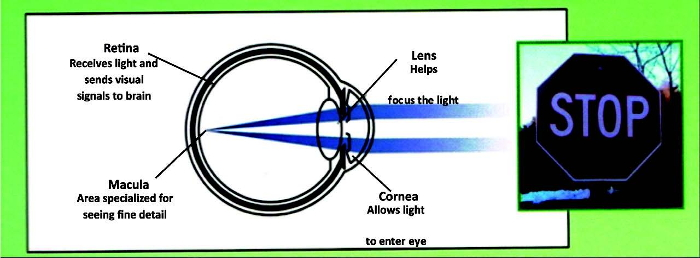
\includegraphics[scale=2.4]{images/049.jpg}
\vskip-.3cm
\end{figure}

Even though the human eye is of the size of a golf ball or smaller, it has several minute structures inside it that perform the functions of a very sophisticated camera. Just as the camera captures light to create a picture on film, the eyes capture light, and transmit these light impulses to the brain to form an image inside the brain.

The anterior or front part of the outer layer of the eye is transpa\-rent and is called the cornea. Its function is to allow light inside the eye, and also to focus light onto the back of the eye. After passing through the cornea, light enters the inside of the eyes via the pupil. As you may have noticed, the size of the pupil can alter to control the amount of light entering the eyes. After passing through the pupil, light encou\-nters the lens, which further helps to focus the light onto the back of the eye. Between the lens and the back of the eye, there is a jelly–like substance called the vitreous. The vitreous helps to maintain the shape of the eye.

At the back of the eye is the all–important retina. The retina is like the film in a camera (not the digital cameras of today, but the SLR came\-ras of the good old days). All light entering the eye is focused onto the retina. The retina has special cells that convert light into ele\-ctrical signals. These signals are sent to the brain via the optic nerve. The brain interprets these electrical signals and forms an image. There is one particular spot on the retina called macula where the vision is extra–sharp. The macula is nourished by tiny blood vessels found both inside the retina, and behind the retina.

So what part of the eye is affected by diabetes? Sadly, diabetes can affect all the structures described above. Hence diabetes is a constant threat to our vision.

\noindent{\textbf{Eye diseases caused by diabetes}}

Now let us discuss the different eye diseases caused by diabetes in order of decreasing magnitude.

\noindent\textbf{\textit{Cataracts}}\index{Cataract}

This is a condition in which the lens inside the eyes becomes\break cloudy, thereby blocking light. The name cataract comes from the Latin word ‘cataracta’, which means waterfall. Just as the water\break rushing down a waterfall appears white, the lens turns white when a cataract deve\-lops. The more severe the cataract, the more opaque the lens becomes. Cataracts are the \# 1 cause of blindness worldwide\break according to the World Health Organization (WHO), accounting for\break 47.8\% of all cases.$^{\text{\cite{chap15–key01}}}$

\begin{figure}[h]
\centering
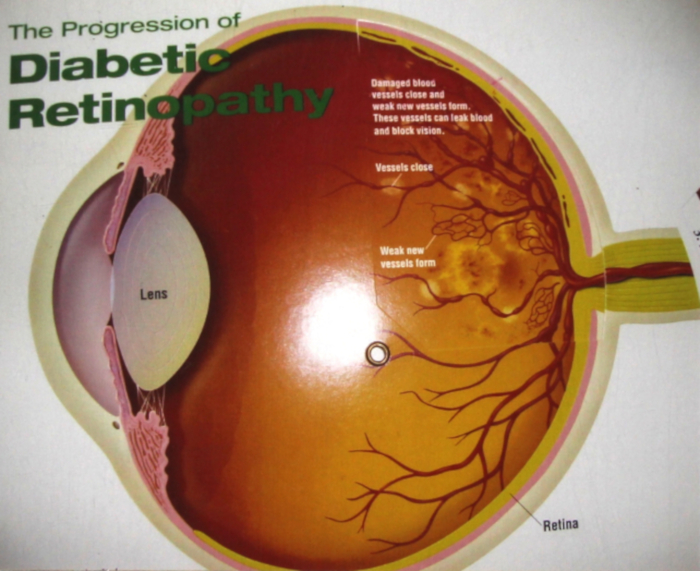
\includegraphics[scale=3.4]{images/050.jpg}
\end{figure}

\textcolor{red}{\textit{People with diabetes are 60\% more likely to develop cataracts than non–diabetics according to the American Diabetic Association. To further complicate matters, diabetics tend to get cataracts at a younger age, and the cataracts in diabetics progress faster.}}

The best way to prevent cataracts is to protect your eyes from the sun’s ultraviolet (UV) rays. According to the United States Environmental Protection Agency (EPA) this can be best achieved by staying indoors during times of strongest UV radiation, namely midday and summer time. Also, be aware that UV rays are reflected by water, sand, etc even if you are in the shade. If you have to go out at these times use of sunglasses and anti–glare lenses for those requiring prescription glasses is advised.

When cataracts are severe, eye specialists can remove the diseased lenses and replace them with new ones. This type of surgery is very common nowadays. But in diabetics this surgery can result in other complications such as glaucoma and retinopathy. Hence, it is best to prevent cataracts in diabetics by means of simple measures described above.

\clearpage
\noindent\textbf{\textit{Glaucoma}}

After cataracts, glaucoma is the 2nd leading cause of blindness\break worldwide accounting for 12.3\% of cases as per the WHO.

Glaucoma is a condition in which there is pressure build–up inside the eyeball. This increased pressure pinches on the optic nerve and the blood vessels that supply the retina. Left untreated, both the retina and the optic nerve sustain damage and result in loss of vision.

\begin{figure}[h]
\centering
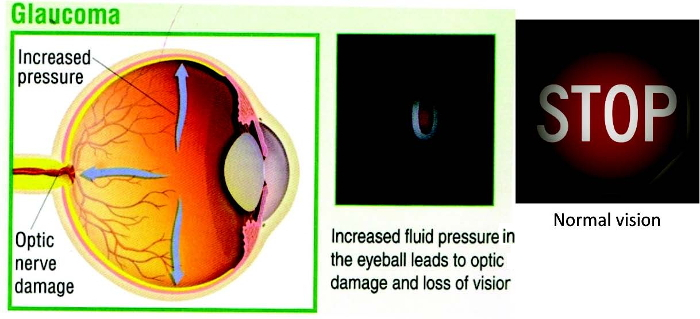
\includegraphics[scale=2.2]{images/051.jpg}
\end{figure}

Diabetics are 40\% more likely to suffer from glaucoma than people without diabetes. The longer someone has diabetes, the greater the chances of developing glaucoma.

\textcolor{blue}{\textit{But glaucoma can be treated with medications or by surgery. The main obstacle to treating glaucoma is not diagnosing it, since in the early stages there are no prominent symptoms. This is one of the reasons why annual eye check–ups and measurement of eye pressure are critical to protect vision in diabetics.}}

\noindent\textbf{\textit{Diabetic retinopathy}}

\begin{figure}[h]
\centering
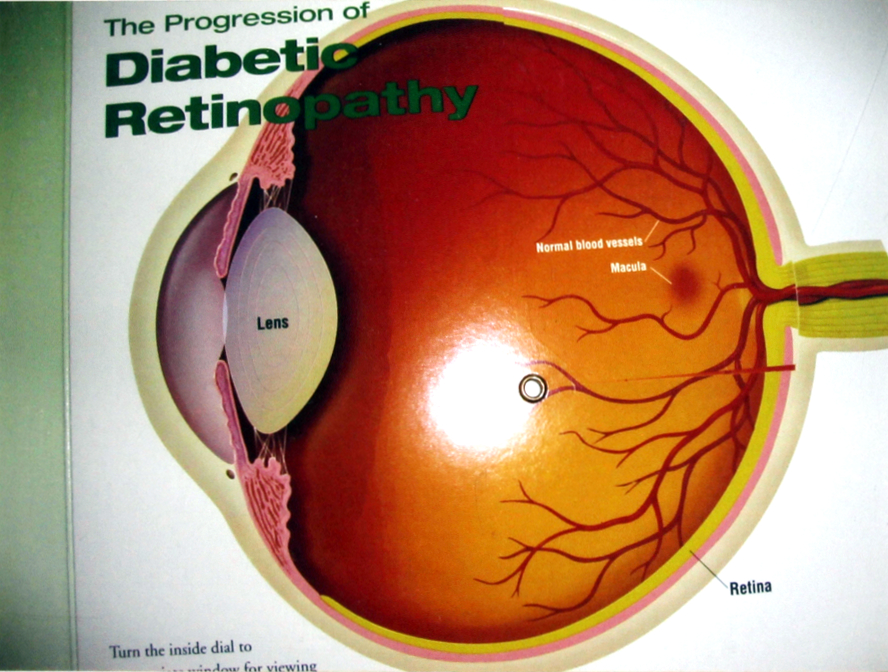
\includegraphics[scale=1.3]{images/052.jpg}\\
\textbf{\textit{Healthy Retina}}
\end{figure}

\begin{figure}[h]
\centering
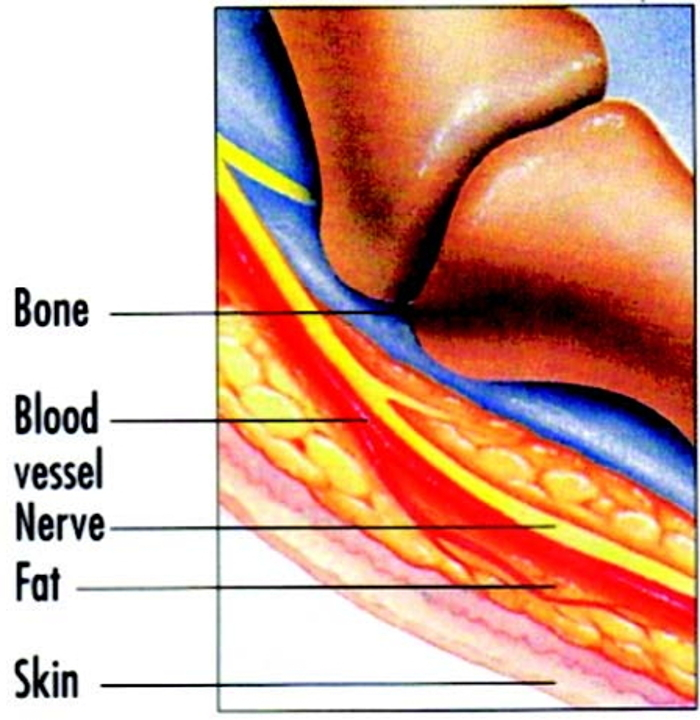
\includegraphics[scale=1.3]{images/053.jpg}\\
\textbf{\textit{Diabetic Retinopathy}}
\vskip-.5cm
\end{figure}

This is a general term for all disorders of the retina caused by\break diabetes. It is the most common of the so–called ‘microvascular\break complications’ of diabetes, the other two being \textit{nephropathy} (kidney\break damage) and \textit{neuropathy} (nerve damage). Microvascular complications refer to diseases that occur as a result of damage to small (or micro) blood vessels.

Most type 1 diabetics develop retinopathy within 20 years of\break having the disease.$^{\text{\cite{chap15–key02}}}$ And type 2 diabetics may begin to develop retino\-pathy as early as 7 years \textbf{before} the diagnosis of diabetes!$^{\text{\cite{chap15–key03}}}$ In the United States it accounts for 10,000 new cases of blindness every year. A study conducted by Sankara Nethralaya in Chennai found that 18\% of diabetics have retinopathy.$^{\text{\cite{chap15–key04}}}$ But this figure was higher (30\%) in a recent study conducted on Indians living in Singapore.$^{\text{\cite{chap15–key05}}}$


\noindent Risk factors for diabetic retinopathy include:

\vspace{-\topsep}
\begin{enumerate}[•]
\itemsep=0pt
\item Poorly controlled diabetes
\item Duration of diabetes– longer the disease, higher the risk
\item Poorly controlled blood pressure
\item Genes
\end{enumerate}

\noindent\textbf{The stages of diabetic retinopathy}

Diabetic retinopathy has four stages:
\begin{enumerate}
\itemsep=0pt
\item Mild Non–proliferative retinopathy
\item Moderate Non–proliferative retinopathy
\item Severe Non–proliferative retinopathy
\item Proliferative retinopathy
\end{enumerate}

\begin{wrapfigure}{l}{6cm}
\centering
\textbf{\textit{Non–proliferative Diabetic Retinopathy}}\\
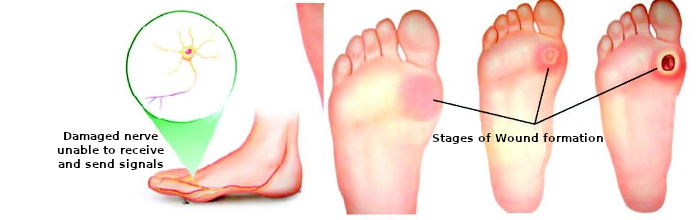
\includegraphics[scale=1.4]{images/054.jpg}
\vskip-.4cm
\end{wrapfigure}

At the root of the pro\-blem lies damage to the walls of the small blood vessels\break supplying the retina. In the early phases the walls of the affe\-cted blood vessels become weak and balloon out to form what are known as ‘micro\-aneurysms’. Fluid can leak from these blood vessels and cause swelling of the retina. If this leakage happens to\break occur at the macula (the site of extra–sharp vision), it\break causes a condition known as ‘macular edema’. This is a dangerous condi\-tion that can lead to permanent vision loss. However, if treated in time, this condition can be reversed.

The microaneurysms can also bleed into the retina and form\break so–called ‘dot hemorrhages’ since they appear like small dots on\break examining the eye.

The changes described up to this stage, namely microaneurysms, macular edema, dot hemorrhages, are all part of the stage described as “non–proliferative retinopathy”. This stage does not result in blindness, except in case of macular edema.

\begin{wrapfigure}{r}{6cm}
\centering
\textbf{\textit{Proliferative Diabetic Retinopathy}}\\
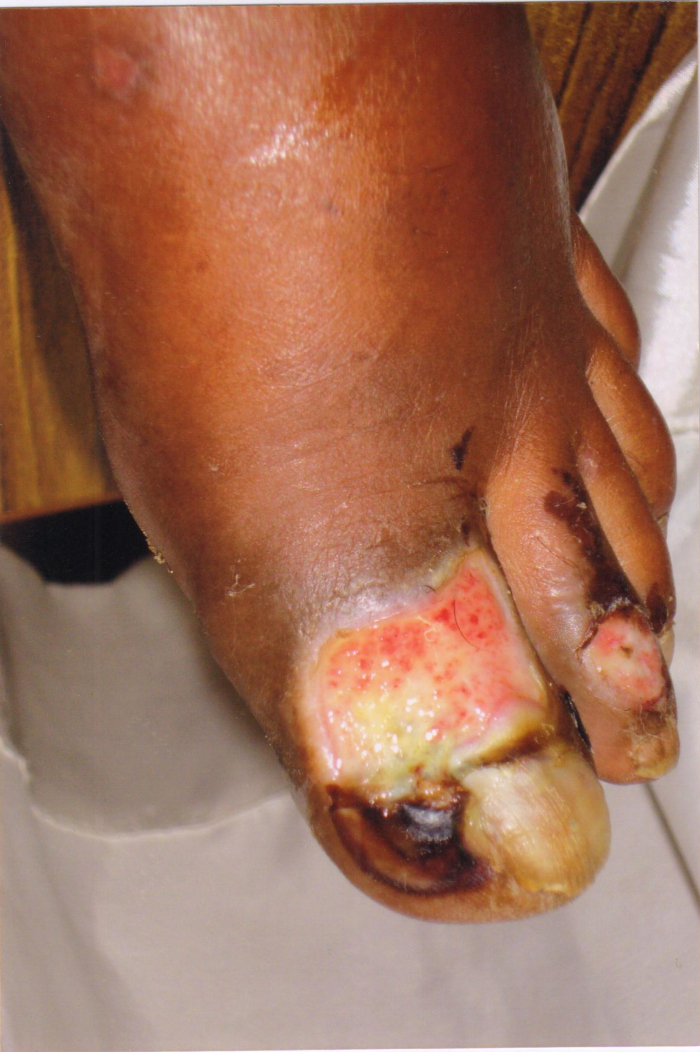
\includegraphics[scale=1.4]{images/055.jpg}
\end{wrapfigure}

Further progression of the disease leads to the next stage called \textit{“proliferative retinopa\-thy”}. During this stage, the damage to the blood vessels continues to the point where they completely shut down. In response, new capillaries or blood vessels start growing into the retina (hence the term ‘proliferative’, since there is a proliferation of new blood vessels). But alas! these new recruits are not as sturdy as the original ones. They are weak, and leak blood into the vitreous, a condition called ‘vitreous hemorrhage’. In addi\-tion, these new blood vessels end up in scar tissue formation in the eye. This scar tissue shrinks over time, and when that happens, it pulls on the retina, causing the retina to\break detach, resulting in ‘retinal deta\-chment’. Both vitreous hemorrhage and \textit{retinal detachment} can cause blindness.

\vskip 4pt
\noindent\textbf{How can diabetic retinopathy be detected early?}
\vskip 4pt

This is possible only by a dilated eye exam by a qualified ophtha\-lmologist.

\vskip 4pt
\noindent\textbf{When should I have my eyes tested for diabetic retinopathy?}
\vskip 4pt

\noindent According to recommendations of the American Diabetes Association:

\vspace{-\topsep}
\begin{enumerate}[•]
\itemsep=0pt
\item If you are between 10 years and 29 years old, and have had diabetes for at least 5 years, you should have dilated eye exams every year.
\item If you are above 30 years of age, you should have annual dilated eye exams. This is regardless of how long you have had diabetes.
\item If you are pregnant or planning to get pregnant, you should have a dilated eye test.
\item If you notice any changes in vision, you should immediately have an eye exam. These changes may include blurry vision, seeing double, seeing spots, trouble reading signs or books, pain or pressure in the eyes, redness of the eyes that does not go away, etc.
\end{enumerate}
\vspace{-\topsep}

\noindent\textbf{Can diabetic retinopathy be treated?}

The answer is a resounding yes. Rapid and huge strides have been made in treatment of this condition. The role of laser has become central in its treatment. Using laser, the ophthalmologist makes tiny burns on the retina. These burns seal the blood vessels and prevent them from leaking and stop them from growing or proliferating. If there is bleeding into the vitreous, then surgery may be done to\break remove the vitreous. If the retina has detached, then it is possible to reattach the retina surgically. The type of treatment depends on the stage of the disease. But the key ingredient for success is early\break detection. The best results are obtained when the vision is still\break normal.

\noindent\textbf{Can diabetic retinopathy be prevented?}

You will be pleased to know that you have considerable control over your own vision, despite having diabetes.

\vspace{-\topsep}
\begin{enumerate}[•]
\itemsep=0pt
\item The single most important intervention on your part to prevent or halt retinopathy is to achieve good diabetes control.
\item Control of high blood pressure.
\item Quitting smoking.
\item Regular eye exams by a qualified ophthalmologist.
\end{enumerate}
\vspace{-\topsep}

\begin{thebibliography}{99}
\bibitem{chap15–key01} Bulletin of the World Health Organization, 2004; 82:844–51.
\bibitem{chap15–key02} UK Prospective Diabetes Study (UKPDS) Group. Intensive blood–glucose control with sulphonylureas or insulin compared with conventional treatment and risk of complications in patients with type 2 diabetes (UKPDS 33). Lancet. 1998; 352(9131):837–53.
\bibitem{chap15–key03} Fong DS, Aiella LP, Ferris FL, \& Klein R. Diabetic retinopathy. Diabetes Care. 2004; 27:2540–53.
\bibitem{chap15–key04} Raman R, Rani PK, Reddi Rachepalle S, Gnanamoorthy P, et al. Prevalence of diabetic retinopathy in India: Sankara Nethralaya Diabetic Retinopathy Epidemiology and Molecular Genetics Study report 2. Opthalmology. 2009; 116(2):311–8.
\bibitem{chap15–key05} Zheng Y, Lamoureux EL, Lavanya R, Wiu R, et al. Prevalence\break and risk factors of diabetic retinopathy in migrant Indians in an\break urbanized society in Asia: The Singapore Indian Eye Study. Opthalmo\-logy. 2012; 119(10):2119–24.
\end{thebibliography}


\chapter{\textit{Diabetic neuropathy}}\index{Diabetic neuropathy}\label{chap16}

A beautiful sunrise, the chirping of birds, the fragrance of flowers, the refreshing taste of morning tea, the cool morning air, are sensations we enjoy everyday, thanks to our nervous system. Each one of these sensations – sight, sound, smell, taste and touch, are conveyed to our brain in the form of electrical signals by our vast nervous system. The brain interprets these signals to create the corresponding sensations.

\textcolor{blue}{\textit{The total length of all the nerves in our body is almost 45 miles! In order to process the vast number of nerve signals, the human brain has more than 1 billion nerve cells called neurons!}} But diabetes can bring this vast empire of communication to its knees.

\vskip 4pt
\noindent\textbf{How does diabetes affect the nerves?}
\vskip 4pt

Excess sugar in the blood damages the tiny blood vessels that\break supply the nerves. As a result the nerves are starved of nutrients\break and oxygen and slowly lose function. This condition is called diabetic\break neuropathy.

\vskip 4pt
\noindent\textbf{What are the factors that increase the risk of diabetic neuropathy?}
\vskip 4pt

Based on currently available scientific research, the following\break factors have been identified:

\vspace{-\topsep}
\begin{enumerate}[•]
\itemsep=0pt
\item Poor glucose control (higher HBA1c level)
\item Longer duration of diabetes (risk increases with disease duration)
\item Age (risk increases with age)
\item Cigarette smoking
\item High cholesterol levels
\item Alcohol intake
\end{enumerate}
\vspace{-\topsep}

\noindent\textbf{How common is diabetic neuropathy?}

\textcolor{red}{\textit{It is the most common complication of diabetes!}} The longer a person has diabetes the higher the probability of having neuropathy. As early as 1 year after having diabetes, about 7\% will have neuropathy. But this number shoots up to 50\% for those with diabetes for more than 25 years.$^{\text{\cite{chap16–key01}}}$

\noindent\textbf{What are the symptoms of diabetic neuropathy?}

The symptoms depend on the type of nerves that are affected. The human body has 3 types of nerves:

\vspace{-\topsep}
\begin{enumerate}
\itemsep=0pt
\item \textbf{Sensory nerves:} These nerves connect our five sense organs (eyes, ears, nose, tongue, skin) to the brain. They receive\break sensory stimuli such as how an object appears (color, shape,\break size, etc) and how it feels (is it soft or firm, hot or cold), or how it smells or tastes.
\item \textbf{Motor nerves:} These nerves help the brain control the various muscles in the body. They carry signals from the brain to our muscles. This enables us to move our different body parts (face, trunk, limbs), and perform various activities such as opening\break and closing our eyes, turning our head, walking, lifting, etc.\break Remember that these nerves are under our conscious control. In other words, they cannot act on their own.
\item \textbf{Autonomic nerves:} These nerves are not under our conscious control. They control the vital functions of our body such as breathing, heartbeat, blood pressure, digestion, sweating, pupil size as it adjusts to light and dark, etc. We have to be extremely thankful to our creator that these vital functions happen on their own. Can you imagine having to remember to breathe 10–15 times every minute, or making our heart beat 72 times per\break minute, every minute of our life!
\end{enumerate}

\noindent In addition to the above classification based on function, nerves can be classified based on their location into:

\vspace{-\topsep}
\begin{enumerate}[a)]
\itemsep=0pt
\item \textbf{Cranial nerves:} These 12 nerves are located in the cranium or the human skull.
\item \textbf{Peripheral nerves:} These nerves are located throughout the\break human body (in the hands, legs, chest, abdomen and pelvis).
\end{enumerate}
\vspace{-\topsep}

Both the cranial and peripheral nerves have a combination of\break sensory, motor and autonomic nerves fibers, and can perform all\break 3 basic nerve functions namely– sensation, muscle control and\break autonomic control.

Diabetes most commonly affects the peripheral nerves, with \textgreater  50\% of all cases of diabetic neuropathy involving peripheral nerves. Among peripheral nerves, the sensory function of the peripheral nerves is most commonly affected. As a result, patients have the following complaints:

\vspace{-\topsep}
\begin{enumerate}[•]
\itemsep=0pt
\item Numbness of feet and hands, which decreases the ability to feel pain, heat and cold. Patients often complain that they feel like they are “walking on cotton”, even if they are walking on a hard surface
\item Tingling and burning sensation in hands and feet. Patients may\break complain that they feel their limbs are “on fire” or someone is\break “poking them with needles”
\item Sharp pains in hands and feet, which are especially worse at night
\item Extreme sensitivity of skin to even light touch.
\end{enumerate}
\vspace{-\topsep}

\noindent Though sensory nerve function is most commonly affected, sometimes the motor function of nerves can also be affected. When this happens, patient may complain of:

\vspace{-\topsep}
\begin{enumerate}[•]
\itemsep=0pt
\item Weakness in the feet and legs
\item Feeling unsteady while standing or walking.
\end{enumerate}
\vspace{-\topsep}

Diabetic neuropathy is often known as “glove and stocking”\break neuropathy, since it commonly affects the hands and feet (parts of the body where gloves and stockings are worn).

The third type of nerve function is autonomic control of the\break vital functions of the body. When this is affected by diabetes, it results\break in a condition known as \textit{“autonomic neuropathy”\index{Autonomic neuropathy}}. This causes many\break debilitating symptoms. These are listed below by the specific organ system affected.

\vspace{-\topsep}
\begin{enumerate}[•]
\itemsep=0pt
\item \textbf{Cardiovascular system}
\vspace{-\topsep}
\begin{enumerate}[o]
\itemsep=0pt
\item Variations in the heart rate, ranging from a very rapid heart rate to a very slow heart rate
\item Variations in blood pressure. This is a serious complication.\break Normally when we stand up from a sitting or lying down\break position, majority of the blood tends to pool in the lower legs due to gra\-vity. As a result, the amount of blood entering the heart\break decreases, and hence less blood is pumped out with each heartbeat. This can cause low blood pressure. But the human body counters this pheno\-menon, by automatically increasing the heart rate, and by compressing the blood vessels of the skin, legs and abdomen, so that the blood is diverted from the skin, legs and abdomen into the heart. But diabetes sabotages this wonderful mechanism. Therefore, diabetic patients with autonomic neuro\-pathy, can feel dizzy when they stand up, and some may even faint!
\end{enumerate}
\item \textbf{Gastrointestinal system}
\vspace{-\topsep}
\begin{enumerate}[o]
\itemsep=0pt
\item The stomach muscles get paralyzed, resulting in nausea, vomiting, bloating, and abdominal pain. This is described in more detail in chapter 19.
\item Bowel habits are affected, causing severe diarrhea at night, or\break severe constipation.
\item Loss of control over the muscles of the anus and rectum, or lack of sensation in this area, may result in embarrassment due to stool accidentally leaking out. This is known as fecal incontinence.
\end{enumerate}
\item \textbf{Urinary system}
\vspace{-\topsep}
\begin{enumerate}[o]
\itemsep=0pt
\item The bladder muscles get paralyzed, and fail to empty the\break bladder, even when the bladder becomes full. As a result, urine may overflow, causing social embarrassment.
\item The bladder muscles may not contract properly to empty the\break bladder completely when urinating. So a small amount of urine is left behind in the bladder, and this creates the urge to urinate again and again.
\item Due to the stagnation of urine in the bladder, there is a higher risk of bladder infections.
\end{enumerate}
\item \textbf{Genital system}
\vspace{-\topsep}
\begin{enumerate}[o]
\itemsep=0pt
\item Men may suffer from impotence (inability to obtain or maintain an erection), while women may suffer from excessive vaginal\break dryness.
\end{enumerate}
\item \textbf{Sweat glands}
\vspace{-\topsep}
\begin{enumerate}[o]
\itemsep=0pt
\item A unique combination of lack of sweating all over the body, but with excess sweating in the face and trunk, can develop. The skin gets excessively dry due to lack of lubrication by sweat. Dry skin is at risk to break down and form ulcers.
\item Excessive sweating while eating, even if the food is not hot or spicy.
\end{enumerate}
\item \textbf{Pupils of the eye}
\vspace{-\topsep}
\begin{enumerate}[o]
\itemsep=0pt
\item The muscles controlling the diameter of the pupils malfunction, and hence the pupil is not able to adjust its size to avoid excess light during the day, and allows more light during the dark, thus affecting vision.
\end{enumerate}
\end{enumerate}

Finally, diabetes can also affect the cranial nerves, or the nerves inside our skull. Most commonly the 3rd and 6th cranial nerves are affected. These nerves control the movements of the eyeball. As a\break result patient often have \textit{diplopia\index{Diplopia}} or “double vision”, due to inability of the two eyeballs to focus on a single object.

\noindent\textbf{What are the complications of diabetic neuropathy?}

The most dreaded complication is a foot ulcer requiring foot or leg amputation. This is explained in detail in the following chapter on\break diabetic foot complications.

\begin{thebibliography}{99}
\bibitem{chap16–key01} Pirart J. Diabetes mellitus and its degenerative complications: A prospective study of 4,400 patients observed between 1947 and 1973. Diabetes Care. 1978; 1:168–88.
\end{thebibliography}


\chapter{Diabetic Foot Disease}\label{chap17}

\vspace{-\topsep}
The feet are at the core of human evolution. We must all be very\break thankful to our ancient predecessors who decided to climb down from\break their tree habitats, and walk on two feet! This freed up our hands to\break channelize our ever–increasing creativity and invent tools and\break technology, as we continued to evolve over millions of years. But this evolutionary adaptation also brought with it unique challenges for the human feet. Our feet now have to bear our entire body weight, and hence the bones and other supporting structures of the feet are prone to wear and tear related damage. We make this worse by wearing\break ill–fitting footwear.

Diabetes exploits this vulnerability by causing ulcers, infections, and bone damage in the feet. This is loosely termed \textit{“Diabetic Foot\break Disease”\index{Diabetic foot disease}}.

\begin{wrapfigure}{r}{4.5cm}
\vskip -.4cm
\centering
{\small\textbf{\textit{Skin and fat form a protective “cushion” that absorbs pressure and protects your foot from infection}}}\\
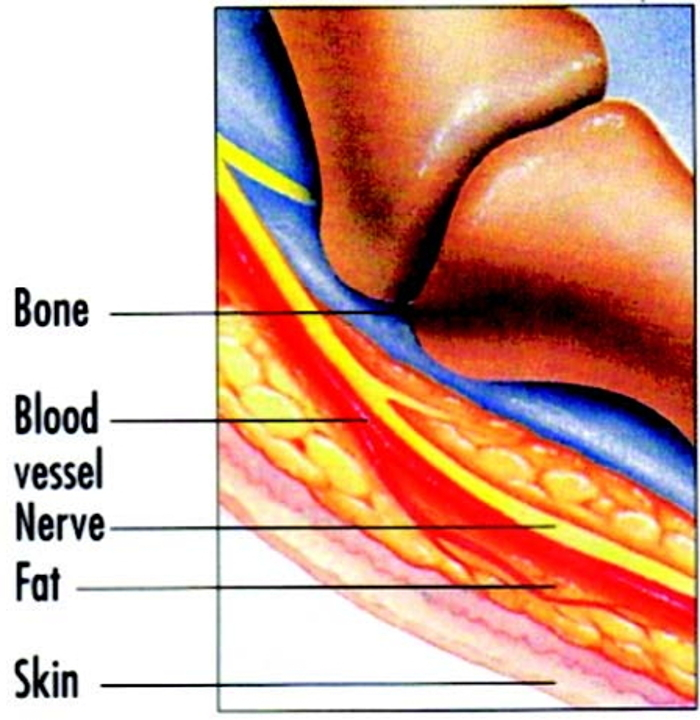
\includegraphics[scale=.8]{images/056.jpg}
\end{wrapfigure}

Of all the complications diabetes causes, foot complications tend to get the least attention. It is but expected that people would be more concerned about their heart, eyes or kidneys, than their feet. But did you know that foot\break complications are the most expensive\break of all diabetes complications! A study from Chennai found that diabetic patients with foot complications spent 32.3\% of their total income toward treatment. In comparison, diabetics with healthy feet spent 9.3\% of their total income on treatment.$^{\text{\cite{chap17–key01}}}$

Diabetic foot infection is the most common reason a person\break with diabetes gets admitted to the hospital.$^{\text{\cite{chap17–key02}}}$ In fact, a diabetic patient\break with foot infection is 55–155 times more likely to require a hospital admi\-ssion compared to a diabetic patient without a foot infection.$^{\text{\cite{chap17–key03}}}$ Up to 75\% of all lower limb amputations are caused by diabetes.$^{\text{\cite{chap17–key04}}}$

This problem is further magnified in India because of our incli\-nation to walk bare foot, either because of religious reasons and/or economic reasons. Thus, both the rich who walk bare foot for religious reasons, and the poor who cannot afford footwear, can be affected. Add to this the poor conditions of our roads, and the risk of foot injury and infection further increases, especially if walking bare foot.

\noindent\textbf{How does diabetes cause foot disease?}

\noindent Diabetes creates some unique situations, which can lead to foot disease.

\vspace{-\topsep}
\begin{enumerate}[i.]
\itemsep=0pt
\item Inability to feel pain: Diabetes causes peripheral neuropathy,\break which predominantly affects the sensory nerves. As a result, the patients cannot feel harmful stimuli such as sharp objects, heat or cold, which damage the skin.
\item Abnormal weight bearing on the foot: This is a consequence of weakness of the foot muscles. Diabetes affects the nerves that control these muscles (diabetic motor neuropathy). Deprived of adequate neural stimulation, the muscles become lazy, lose their strength and shrink in size. With no muscle mass, the foot\break becomes deformed. The weight of the body is now distributed abnormally on the deformed foot, causing increased pressure in certain areas. These high–pressure areas when injured by sharp objects, heat or cold, develop ulcers or wounds.
\item Autonomic neuropathy due to diabetes decreases the blood\break supply to the foot. Thus the foot that is already insensitive and\break deformed is weakened further by lack of adequate oxygen and\break nutrition. This makes it susceptible to injury. In addition, it also struggles to heal after an ulcer or wound forms due to the lack of adequate blood supply.
\item Autonomic neuropathy also leads to decreased sweating in the skin of the foot. The skin turns dry and cracks, and fissures develop through which bacteria can enter and cause foot infections.
\end{enumerate}

\begin{figure}[h]
\centering
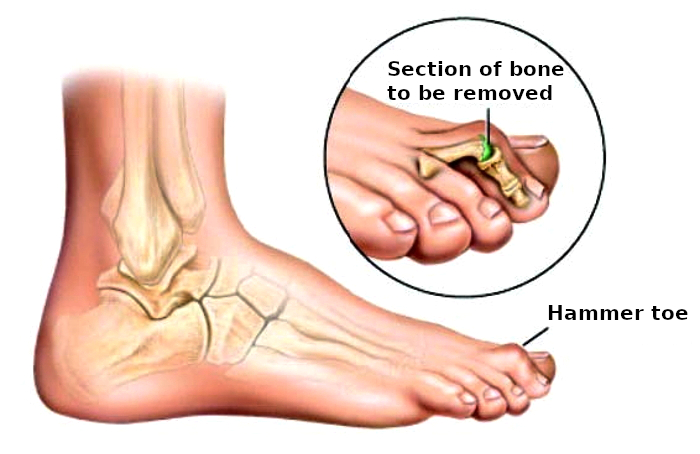
\includegraphics[scale=2.3]{images/057.jpg}
\vskip-.1cm
\end{figure}

\noindent\textbf{What are the two main foot diseases caused by diabetes?}

\vspace{-\topsep}
\begin{enumerate}
\itemsep=0pt
\item Diabetic foot ulcer
\item \textit{Charcot’s joint\index{Charcots joint}}
\end{enumerate}

\noindent{\textbf{What is diabetic foot ulcer?}}

\begin{wrapfigure}{r}{4.5cm}
\centering
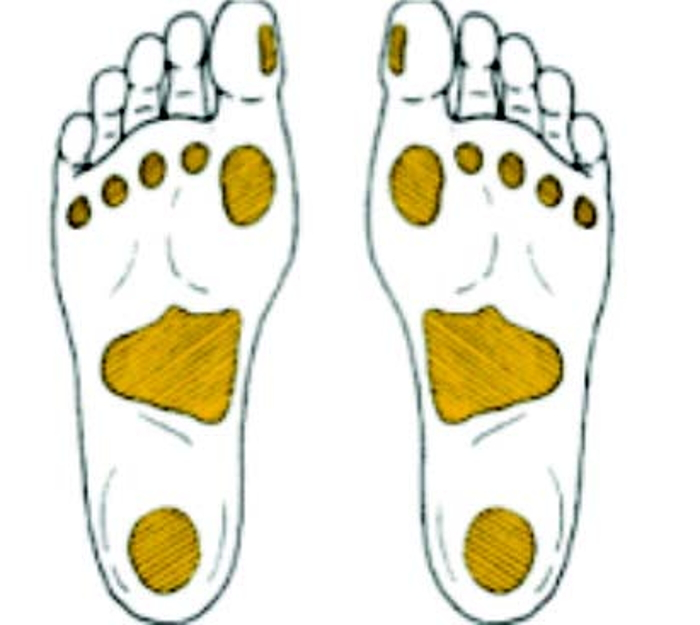
\includegraphics[scale=.8]{images/058.jpg}\\
\textbf{\textit{Diabetic foot ulcer}}
\vskip-.5cm
\end{wrapfigure}

Diabetic foot ulcer is a major compli\-cation of diabetes. Up to 15–25\% of all patients with diabetes will have this complication at some point in their life. When the foot is affected, the person is unable to perform his job, and often loses his source of income. This affects the entire family both economically and psychologically. Once formed, the ulcer heals very slowly due to lack of adequate blood supply or nutrition to this area, as the blood vessels in this area are also affected by diabetes. Even if the ulcer heals, there is a high risk of it recurring. \textcolor{red}{\textit{This is probably the single most common reason for leg amputations.}} In severe cases, the ulcer can get infected, and this infection can spread throughout the body and poison us to death!

But this is not something that happens overnight. \textcolor{blue}{\textit{It comes with suffi\-cient warning, and there are several simple interventions that\break can prevent this frightful complication. But first we need to understand the\break different stages of this disease.}}

\noindent{\textbf{First stage of the disease}}

This is the dawn of the disease. There is no break in the skin, but the necessary ingredients to launch an assault on the skin have assembled. These include:

\begin{center}
\begin{tabular}{@{}ccc@{}}
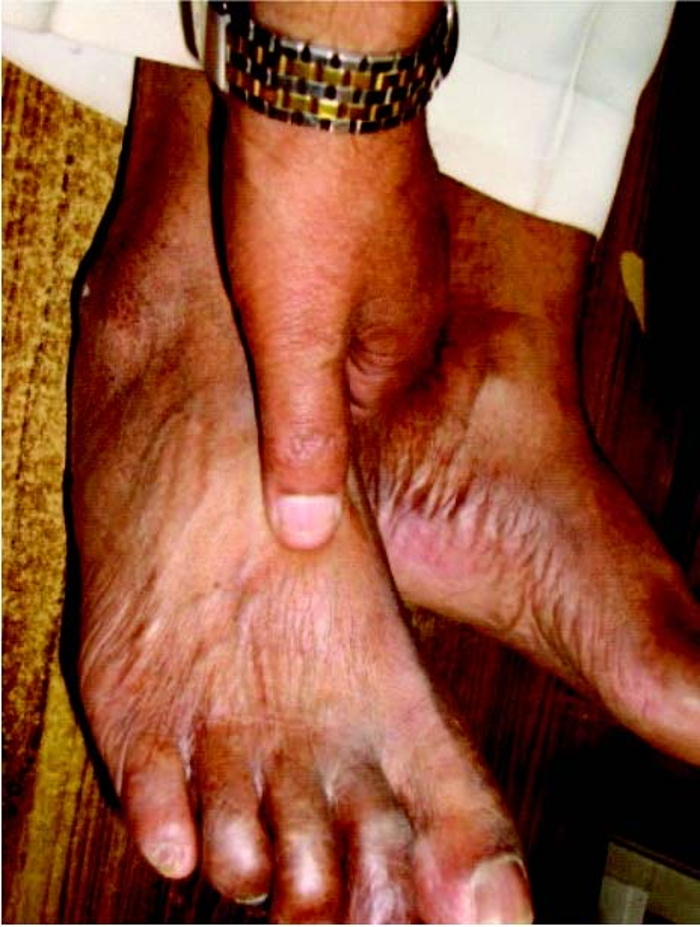
\includegraphics[scale=.7]{images/060.jpg} &
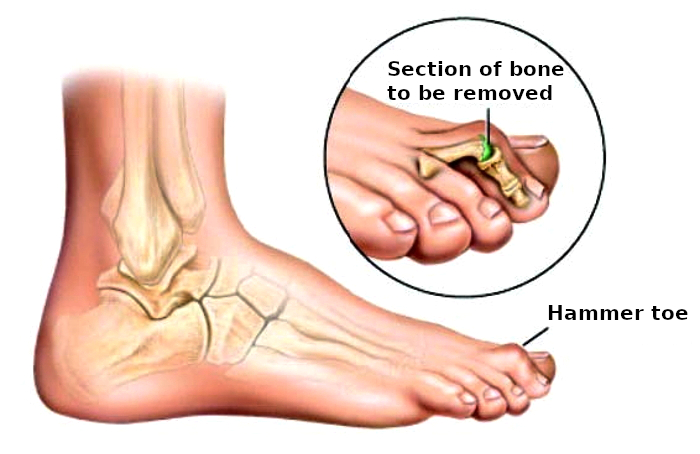
\includegraphics[scale=.8]{images/061.jpg} &
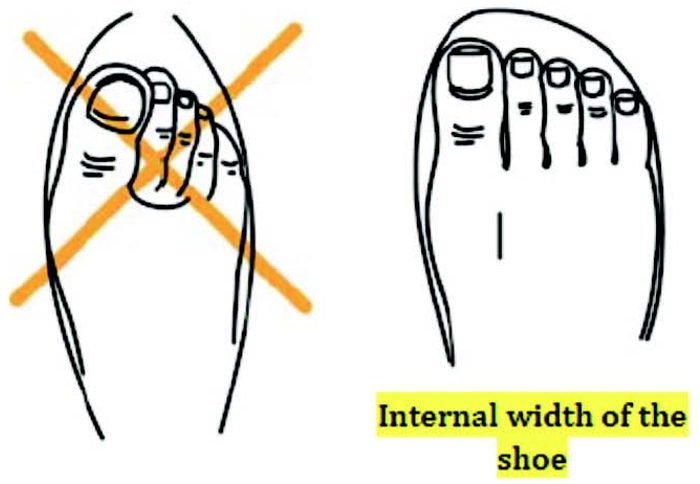
\includegraphics[scale=.8]{images/062.jpg}
\end{tabular}
\end{center}

\begin{enumerate}[a.]
\itemsep=0pt
\item Skin abnormality– dry skin (due to lack of sweat), callus formation.
\item Bone deformity – such as hammer toe, etc.
\item Joint deformity– Charcot joint (this is explained in detail later).
\item Nerve problems – diabetic peripheral neuropathy, motor neuro-\break pathy, autonomic neuro\-pathy.
\item Decreased blood flow– due to atherosclerosis and autonomic neuro\-pathy.
\end{enumerate}

This stage offers several early warning signs, which if identified and acted upon, can prevent the potentially gruesome outcomes of\break diabetic foot ulcer such as amputation and death.

\begin{figure}[h]
\centering
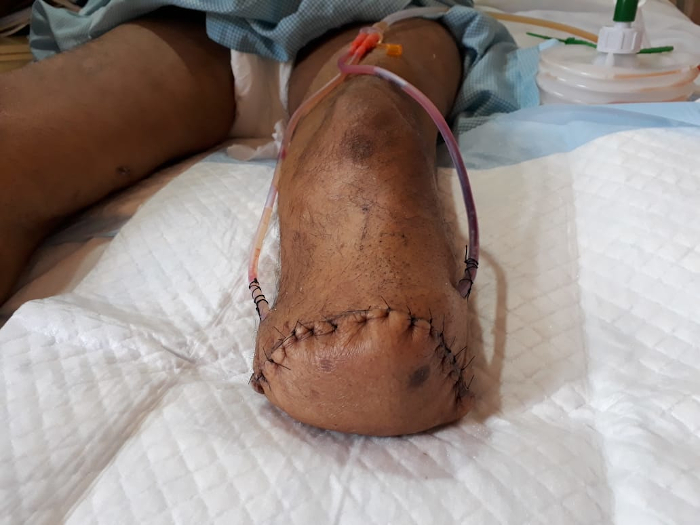
\includegraphics[scale=2.3]{images/062a.jpg}\\
\textbf{\textit{Knee amputation stump, wound looks healthy}}
\end{figure}

\noindent\textbf{How can we identify these early warning signs?}

This does not require any expensive tests. The following simple and easy methods can help:

\vspace{-\topsep}
\begin{enumerate}[i.] 
\itemsep=0pt
\item Inspecting the feet daily, especially in between toes and the\break soles, will alert us to skin changes (dry, cracked, fissured, callus\break formation), and foot deformities (hammer toe, loss of muscle mass). You should definitely have your doctor check your feet during your consultation or clinic visit.
\item Early detection of nerve damage in the feet by your doctor by using a tuning fork or a monofilament.
\item Early detection of decreased blood supply to the feet by your doctor by feeling the pulse in your feet.

\clearpage

\begin{center}
\begin{tabular}{@{}c@{}}
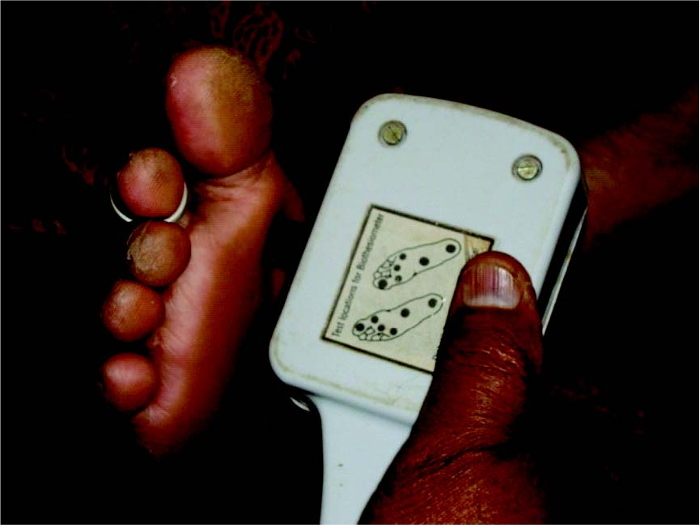
\includegraphics[scale=.9]{images/063.jpg}\\
{\small\textbf{\textit{Early detection of nerve damage in the}}}\\
{\small\textbf{\textit{doctor's office by Vibrotherm test}}}
\end{tabular}
\end{center}
\end{enumerate}

\noindent\textbf{Once we know that the foot is at risk for an ulcer due to diabetes, what measures can be taken to prevent an ulcer from developing?}

\begin{figure}[h]
\centering
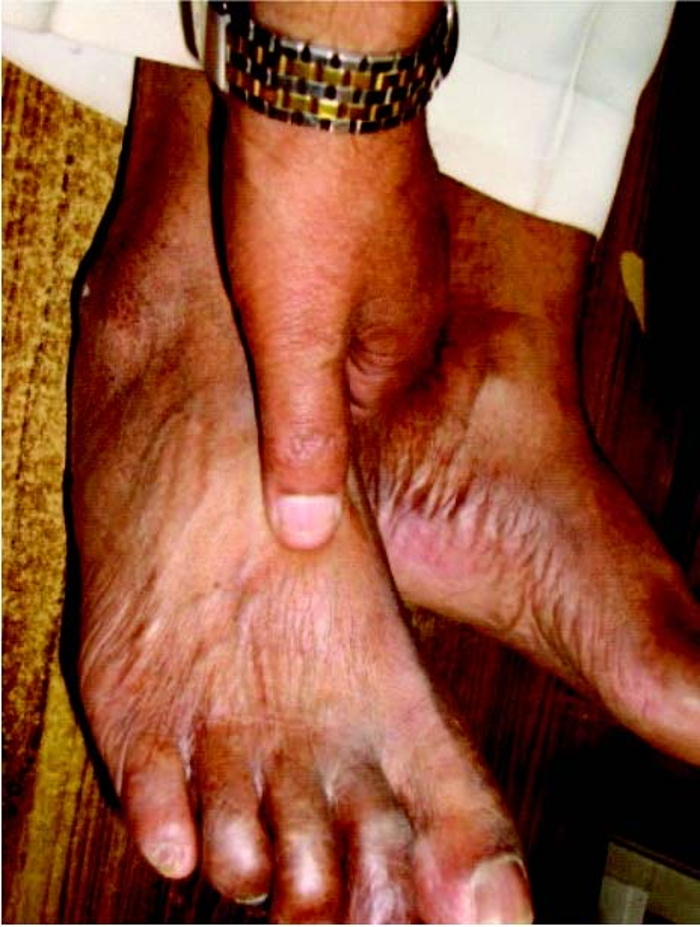
\includegraphics[scale=.9]{images/064.jpg}\\
\textbf{\textit{Detecting decreased\\ blood supply}}
\end{figure}

A few basic common sense measures can go a long way in preve\-nting serious complications of diabetic foot. These include:

\vspace{-\topsep}
\begin{enumerate}[a.]
\itemsep=0pt
\item Apply skin lotions or moisturizers to prevent cracking and fissuring that can develop due to dry skin.
\item Clip nails regularly.
\item Wearing the right fitting shoes. Sometimes, people with diabetes may need custom–fit shoes. As previously mentioned,
 \begin{figure}[h]
\centering
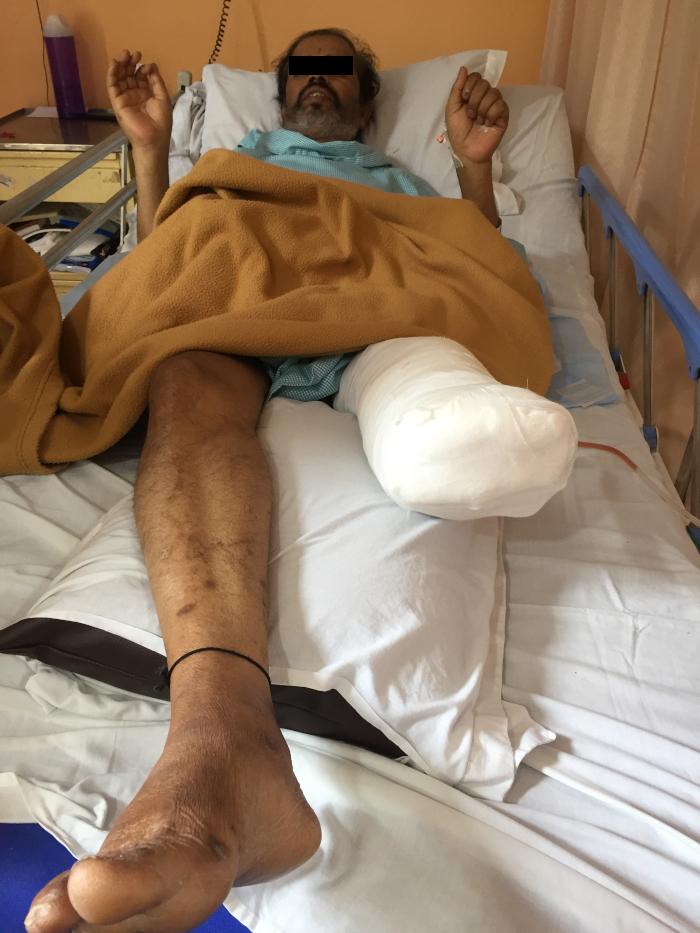
\includegraphics[scale=.8]{images/065.jpg}
\end{figure}
many\break diabetics have deformed feet. Just as you have your tailor stitch shirts or trousers that are the right fit for you, shoes may also need to be specially designed for the exact shape and size of your feet to prevent creating areas of excess pressure in your feet. In fact, there are many companies that specialize in building custom footwear for\break diabetics.
\item Avoid wearing shoes for prolonged periods of time. This can cause sustained pressure on certain parts of the foot, and can lead to\break ulcers. It is recommended to remove shoes every 4 hours, inspect the feet, and to stretch the feet.
\end{enumerate}
\vspace{-\topsep}

If you follow the above reco\-mmenda\-tions, you will be able to not only save your feet, but even your life!

\begin{wrapfigure}{r}{4.5cm}
 \vskip -.4cm
\centering
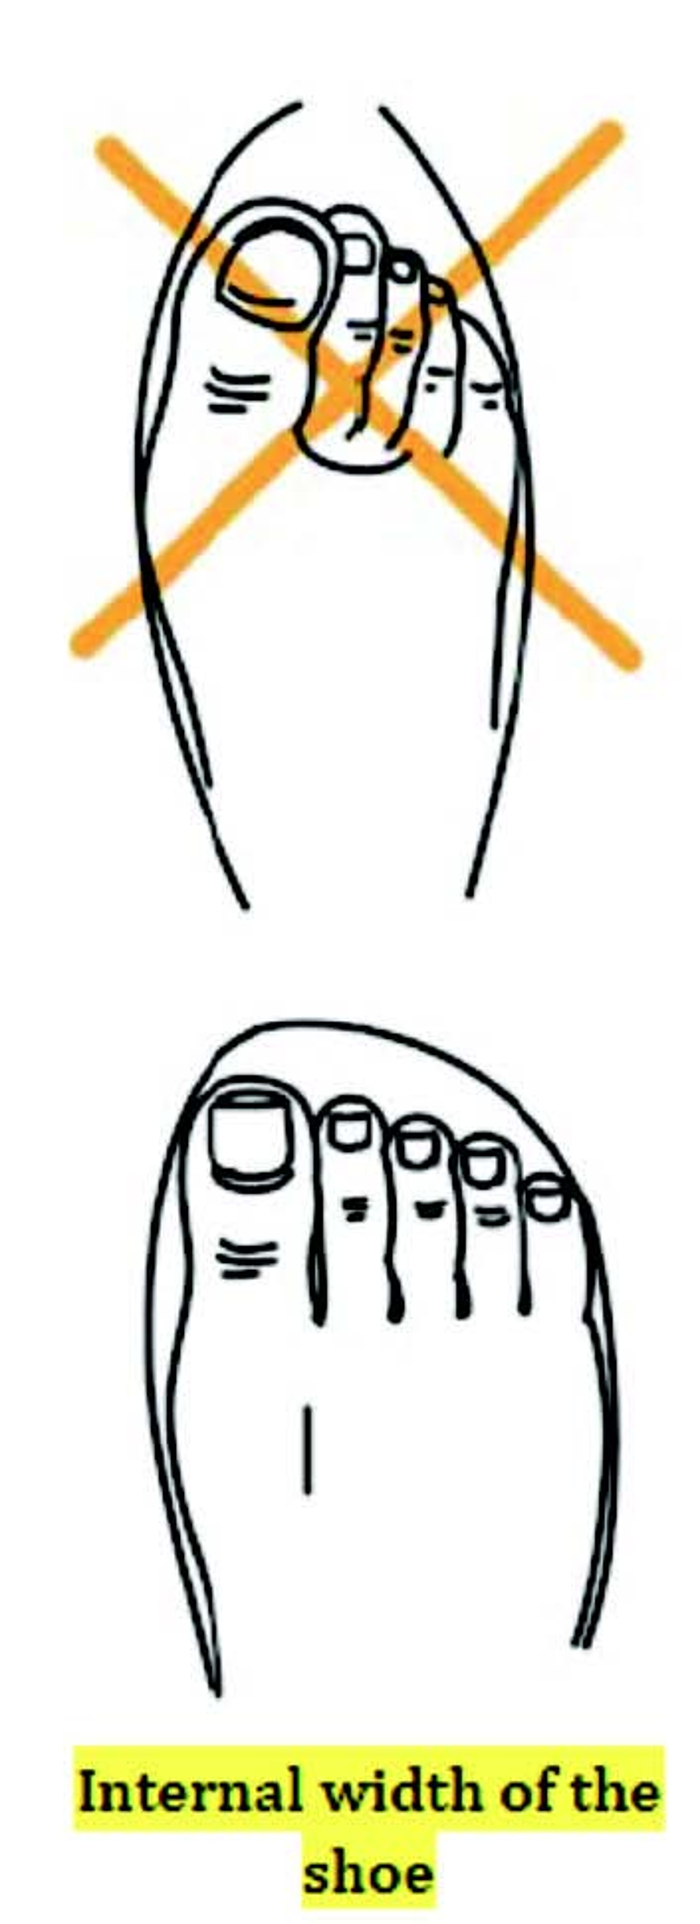
\includegraphics[scale=.5]{images/066.jpg}
 \vskip -.4cm
\end{wrapfigure}

\noindent{\textbf{Second stage of diabetic ulcer}}

Unfortunately, many diabetics in our country have progression of foot disease due to lack of awareness, and lack of proper medical care. Hence, they can deve\-lop the second stage of\break diabetic foot ulcer.

In this stage, the skin that had a\break callus in the first stage later develops a\break superficial ulcer. Unless treated pro\-perly, the ulcer spreads deeper into the foot.

\clearpage

\vspace{-\topsep}
\noindent\textbf{Treatment}
\begin{enumerate}[•]
\itemsep=0pt
\item Removing the dead skin at the site of the ulcer, to enable healthy tissue to grow back.
\item Avoiding weight bearing on the affected foot to prevent pressure points, because this will delay healing. This can be done by using a walker or crutches, and in some cases, special casts and foam\break dressings.
\item Changing dressings daily.
\item Administering antibiotics if the ulcer is infected.
\item Surgery to correct the foot deformity may be necessary if the ulcer(s) keep coming back.
\end{enumerate}

\begin{figure}[h]
\centering
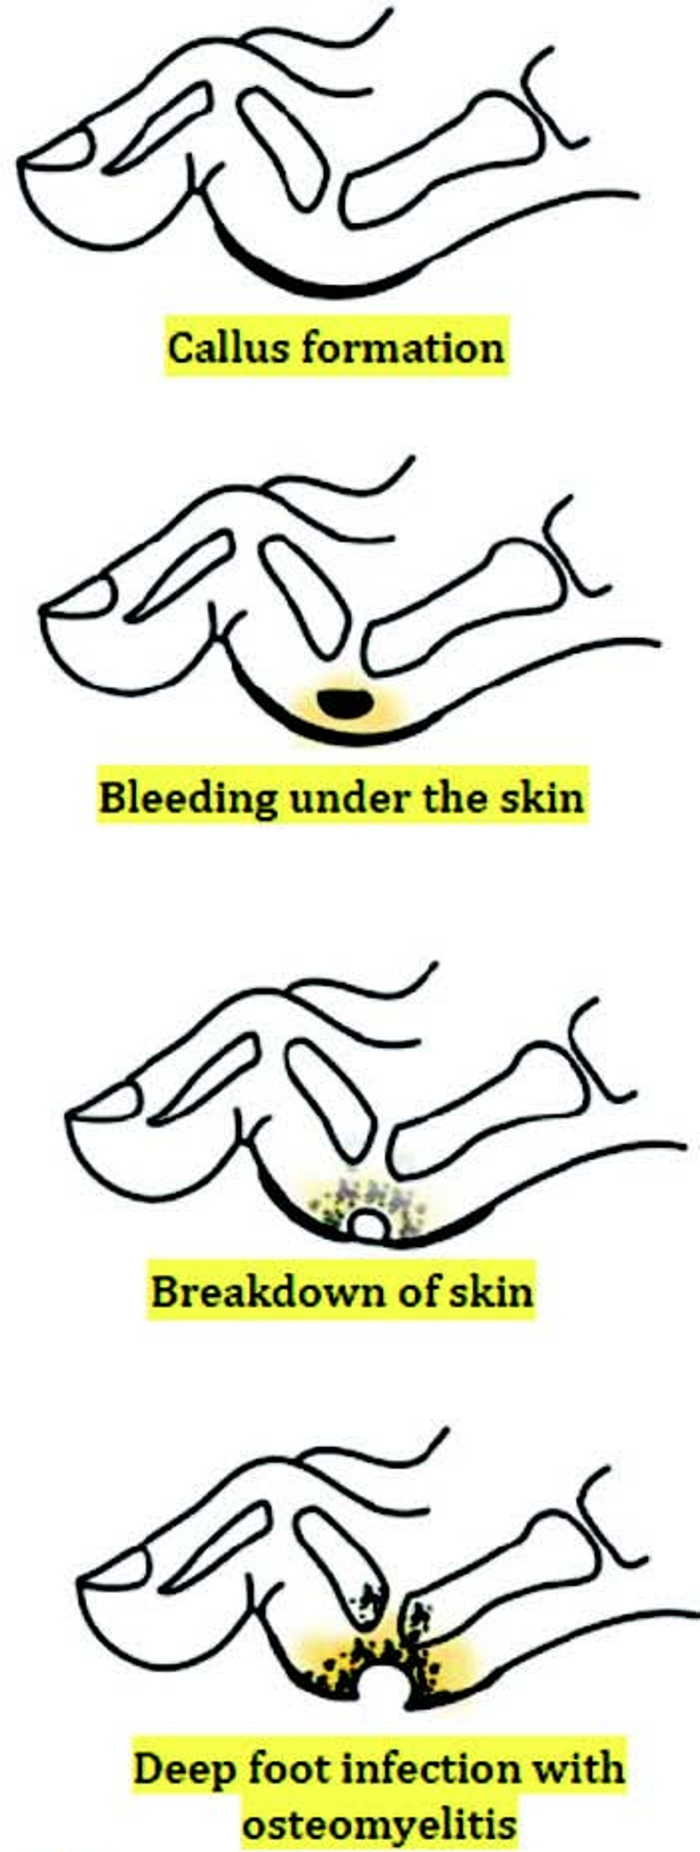
\includegraphics[scale=2.4]{images/067.jpg}\\
\textbf{\textit{Illustration of ulcer due to repetitive stress}}
\end{figure}

\noindent{\textbf{Stage 3 of the diabetic ulcer}}

If stage 2 is not identified or addressed correctly, the superficial ulcer that was only involving the skin spreads deeper to involve the tendons and joint coverings (called joint capsules).

\noindent{\textbf{Stage 4 of the diabetic ulcer}}

The ulcer now has crossed the skin and tendons, to involve the bone.

At this stage treatment is much more aggressive. Not only is the dead skin removed, but sometimes even the infected bone has to be removed. Most of the treatment has to be done in the hospital, sometimes even by a surgeon in the operating room. Antibiotics are frequently given through the veins to control infection in the ulcer.

\clearpage

\noindent{\textbf{Stage 5 of the diabetic ulcer – \textit{Diabetic gangrene\index{diabetic gangrene}}}}

This is the most serious stage of the disease, and can easily cost a person his life!

Gangrene is derived from the Latin word \textit{“gangraena”} and the Greek word \textit{“gangraina”}, both of which mean “death or decay of tissue”.

\noindent\textbf{There are 2 kinds of gangrene– dry and wet.}

In \textbf{dry gangrene}, the chief cause of tissue death is lack of oxygen and nutrients. The entire human body is supplied with oxygen and\break nutrients by a constantly flowing stream of blood through the arte\-ries. But diabetes damages these vital lifelines. The arteries get clogged\break inside, and the nerves controlling the arteries are damaged as\break well (auto\-nomic neuropathy). In this context, minor injuries such as\break pun\-cture wounds, abrasions, etc, fail to heal well, because the\break damaged tissue is not getting adequate oxygen and nutrients. This causes the tissue to eve\-ntually die of starvation from both oxygen and food. Eventually the dead part of the foot will fall off on its own, a phenomenon known as “autoamputation”.

In \textbf{wet gangrene}, the chief cause of tissue death is overwhel\-ming infection. Bacteria creep into the feet of diabetics through cracks and fissures in the skin. The oxygen–deficient environment due to decrea\-sed blood supply in the feet of diabetics provides a fertile breeding ground for bacteria. They multiply in large numbers and clog up the veins. Veins are in charge of carrying blood back to the heart from the various parts of the body. When they are blocked, blood stagnates in tissues and promotes bacterial growth. In response to this, the body sends its soldiers (the white blood cells) to fight the bacteria. In this fight a large number of bacteria and white blood cells die, and the fluid content of these cells spill out. The swelling that results from this leakage increases the pressure in this area. This increased pressure squeezes the already damaged blood vessels. Thus, the blood supply to this area gets completely cut off, and results in more cell death.

\clearpage

The stagnant blood and fluids leaking from dead cells causes a\break ‘wet’ gangrene. This type of gangrene is much more dangerous than\break dry gangrene. The bacteria produce large amounts of toxins, which can spread throughout the body via blood, and cause a toxic shock resu\-lting in death.

\begin{center}
\begin{tabular}{@{}cc@{}}
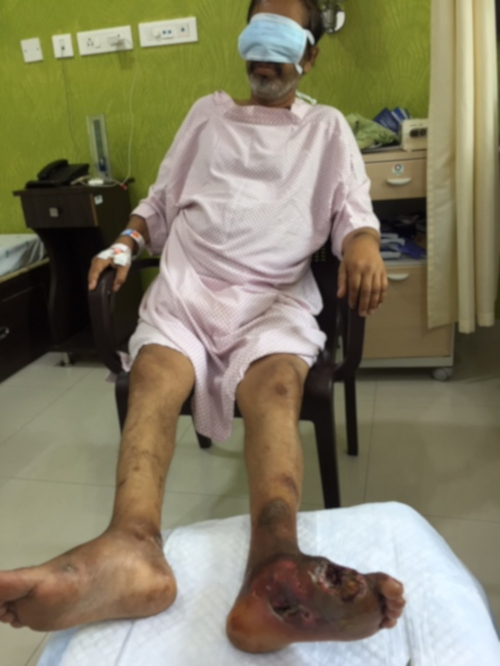
\includegraphics[scale=1.1]{images/068.jpg} &
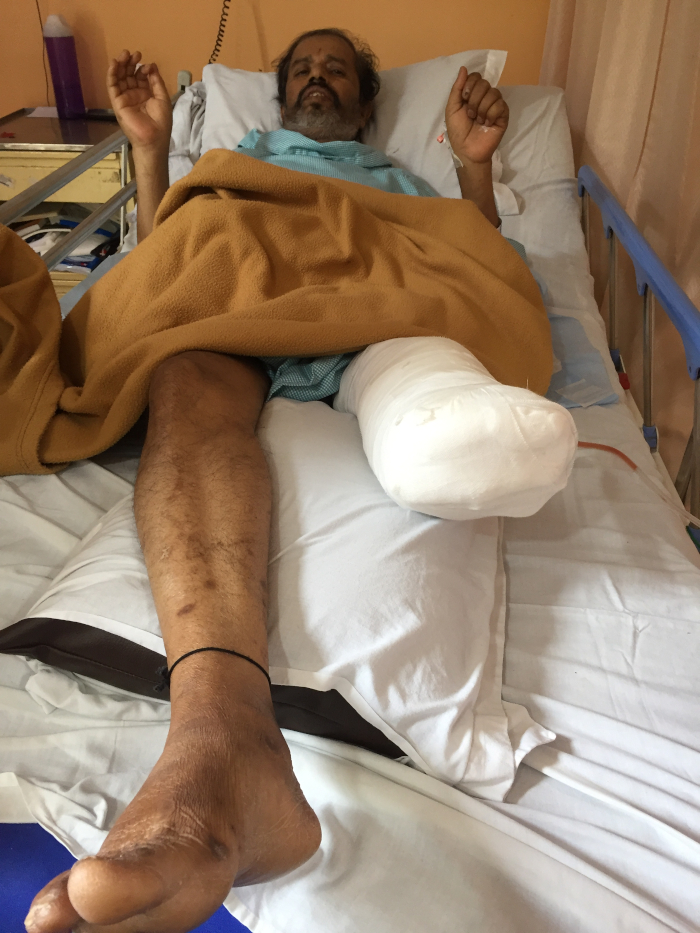
\includegraphics[scale=1.1]{images/068a.jpg}
\end{tabular}
\end{center}

Gangrene is a medical emergency! Immediate surgery is required to remove the dead tissues where bacteria are breeding and manu\-fa\-cturing life–threatening toxins. This often requires amputations of the feet and in some cases the entire limb, in order to save the rest of the body.

The following pictures of diabetic gangrene are from a 65–year old patient of mine, with a 15–year history of diabetes. He was also a chain smoker. He had recently spent a lot of time driving to and in Bengaluru. He had developed a small callus with surrounding redness in the right sole. He had a fever. This was a sign of infection. Though he was advi\-sed immediate care at the hospital, he refused. He went home with antibiotics, promising to come back the next day. But his fever got worse the next day and he was too sick to leave home. On the third day i.e. 48 hours later, his right foot was gangrenous. He had to be rushed to the hospital for foot surgery. Eventually with insulin, antibiotics, dressing changes and rest, he recovered well, but had lost a part of his foot forever.

\noindent\textbf{Diabetic foot ulcer in India}

A study comparing patients with diabetic foot disease in Germany and in India showed that 48\% of German patients had pro\-blems with 
\begin{wrapfigure}{r}{5cm}
\centering
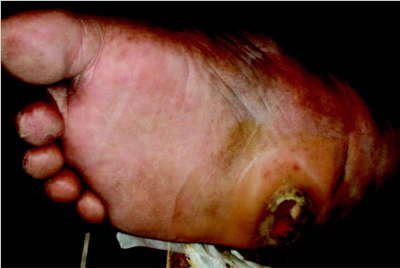
\includegraphics[scale=.6]{images/069.jpg}\\
\textbf{\textit{Day 1 – Ulcer right foot}}
\vskip-.3cm
\end{wrapfigure}
blood vessels in the foot, but only 13\% of Indian patients had problems with blood supply.$^{\text{\cite{chap17–key05}}}$ There is also scientific evidence that shows that Indians are less affected by diabetic neuropathy than Caucasians. But still many diabetics in India fall victim to diabetic foot ulcers. There are some unique social and cultural\break behaviors to explain this:

\begin{figure}[h]
\centering
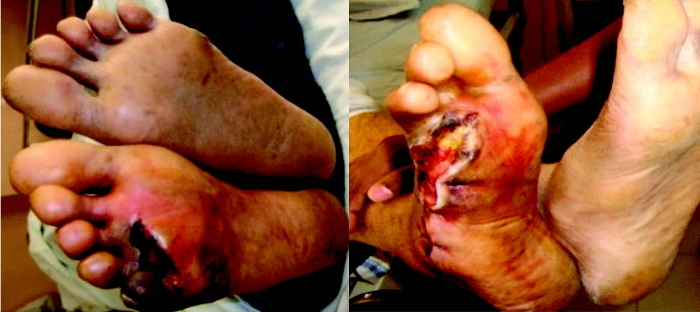
\includegraphics[scale=1.6]{images/070.jpg}\\
\textbf{\textit{Day 3 – Wet gangrene   After partial amputation}}
\vskip-.5cm
\end{figure}

\begin{enumerate}[•]
\itemsep=0pt
\item Walking barefoot while going to temples, etc exposes the feet to sharp objects like stones, etc. Also bacteria in the dust and soil get a chance to enter the feet through skin breaks.
\item Walking barefoot over hot coals is a religious tradition in some part of the country. This causes severe burns and injury to the feet.
\item Some of my patients have lost their feet.
\item Some people refrain from wearing footwear made of leather to\break temples.
\item Many living in poverty cannot afford to wear footwear !
\end{enumerate}
\vspace{-\topsep}

\noindent{\textbf{\textit{Charcot joint\index{Charcots joint}}}}

This is a strange and debilitating complication of diabetes that\break affects the joints. Jean–Martin Charcot, a French neurologist, first\break described it in 1868.

\begin{wrapfigure}{l}{5cm}
\centering
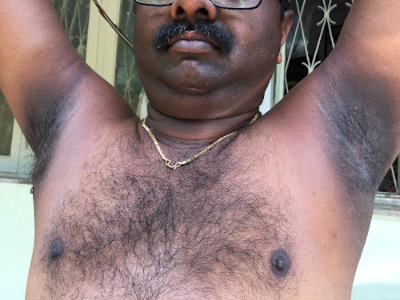
\includegraphics[scale=1.7]{images/071.jpg}\\
\textbf{\textit{Charcot foot}}
\vskip-.5cm
\end{wrapfigure}

In nature there is a harmony between creation and destruction. When there is too much creation (like our population) or too much destruction (like our environment), it leads to problems. The same is true of our bones. There is creation or laying down of new bone by one type of cells (called osteoblasts), and this new bone is remodeled to remove excess or faulty bone by another type of cells (called osteoclasts). There is an imbalance between bone formation and bone remodeling in Charcot joint or Charcot foot.

The most commonly affected joint (60\% of all cases) is located in the front part of the foot (tarso–metatarsal joint). Other joints commonly involved are the joints between the fingers and the hand (metata\-rso\-pha\-la\-ngeal) in 30\% cases, and the ankle joint in 30\% of cases.

The condition usually presents as a red, swollen, warm foot or\break ankle. Astonishingly, despite all this swelling and redness, the patient does not feel any pain!

Underneath these skin changes, the joint is being destroyed. If this continues, the whole joint becomes severely deformed, and the skin overlying the joint gets ulcerated. Due to delays in diagnosis or wrong diagnosis, more than half of these patients will develop an ulcer, and eventually this will need an amputation.

\begin{thebibliography}{99}
\bibitem{chap17–key01} Shobhana R, Rao PR, Lavanya A, Vijay V, \& Ramachandran A. Cost burden to diabetic patients with food complications– A study from southern India. J Assoc Physicians India. 2000; 48 (12):\break 1147–50.
\bibitem{chap17–key02} Lavery LA, Armstrong DG, Wunderlich RP, Tredwell J, \& Boulton AJ. Diabetic foot syndrome: Evaluating the prevalence and incidence of foot pathology in Mexican Americans and non–Hispanic whites from a diabetes disease management cohort. Diabetes Care. 2003; 26 (5): 1435–8.
\bibitem{chap17–key03} Lavery LA, Armstrong DG, Wunderlich RP, Mohler MJ, et al. Risk factors for foot infections in individuals with diabetes. Diabetes Care. 2006; 29 (6): 1288–93.
\bibitem{chap17–key04} Viswanath V. The diabetic foot: Perspectives from Chennai, South India. Inj J Low Extrem Wounds. 2007; 6 (1): 34–6.
\bibitem{chap17–key05} Morbach S, Lutale JK, Viswanathan V, Mollenberg J, et al. Regional differences in risk factors and clinical presentations of diabetic foot lesions. Diabet Med. 2004; 21 (1): 91–5.
\end{thebibliography}

\newpage
 
\renewcommand{\thechapter}{\arabic{chapter}A}
\chapter{Skin Disease and diabetes}\label{chap18A}

The skin is the largest organ in our body with a total surface area of two square meters. Up to 30\% of all diabetics suffer from some form of skin disease according to the American Diabetes Association. The skin condition may either be a direct consequence of diabetes, or a common condition that can affect anyone, but which is made worse by diabetes. While in general, skin conditions in diabetes are not very dangerous, they can lead to dangerous complications if not managed promptly (such as diabetic foot and gangrene). Also one type of skin condition could lead to another (for example dry skin can lead to skin infections).

\vskip 4pt
\noindent The following table lists commonly seen skin conditions in diabetics:

\begin{center}
\begin{tabular}{|l|l|}
\hline
\multicolumn{1}{|c}{\textbf{Skin conditions made}} & \multicolumn{1}{|c|}{\textbf{Skin conditions caused}}\\
\multicolumn{1}{|c}{\textbf{worse by diabetes}} & \multicolumn{1}{|c|}{\textbf{by diabetes}}\\
\hline
Itching & Diabetic dermopathy\\
\hline
Bacterial infections- usually- & Necrobiosis\\
staphylococcal & \\
\hline
Fungal infection- usually candidal & Blisters\\
\hline
Athlete’s foot, ringworm, jock itch & Eruptive xanthomatosis\\
\hline
\end{tabular}
\end{center}

\noindent{\textbf{Skin itch and diabetes}}

This is a very common problem for many diabetics. In some dia\-betics the itching is so severe, that they scratch to the point where they inflict many wounds on their own skin, and cause severe dis\-coloration of the skin. This can lead to poor self–image, because of which\break people avoid social gatherings or going out of their homes. It is not un\-common to have severe depression because of this.

So what is the cause of this severe itching among diabetics? Itching in diabetes has several underlying causes as described below:

\vspace{-\topsep}
\begin{enumerate}[•]
\itemsep=0pt
\item Dry skin: As a result of hyperglycemia, there is excess urination and hence dehydration. This results in dry skin
\item Autonomic neuropathy: Diabetes affects the autonomic nervous\break system that is in charge of stimulating sweat glands. As a result there is less sweating, especially in the lower legs, which again leads to dry skin
\item Poor blood circulation: Diabetes affects the small blood vessels that supply blood to the skin. Itching may actually be the first sign of poor blood circulation in diabetes.
\item Skin infections, especially fungal infections are another cause for skin itching.
\end{enumerate}
\vspace{-\topsep}

\noindent\textbf{Remedies for itchy skin}

\noindent Several simple measures can help prevent and manage this vexing\break problem.

\vspace{-\topsep}
\begin{enumerate}[•]
\itemsep=0pt
\item Use a mild soap (such as Dove)
\item Apply a moisturizing cream immediately after taking a bath or\break washing up, before the skin gets dry
\item Do not apply moisturizer in areas that usually stay moist such as\break between toes, groin, under arms and under the breasts. These areas should be kept dry to prevent fungal infections
\item Apply talc or antifungal powder between skin folds
\item Avoid very hot water because it causes your skin to dry up, and can also cause burns in diabetics who may have poor sensation
\item Good blood sugar control will prevent damage to the nerves and blood vessels, and in turn prevent dry skin and itching.
\end{enumerate}
\vspace{-\topsep}

\noindent{\textbf{Skin infections in diabetes}}

Diabetics are at higher risk for skin infections than the general popu\-lation due to the following reasons:

\vspace{-\topsep}
\begin{enumerate}[•]
\itemsep=0pt
\item There is a higher glucose content in the sweat, which provides\break favorable conditions for microbes (bacteria and fungi) to multiply.
\item The white blood cells, which are responsible for fighting off infe\-ctions, are sluggish when the blood sugar is high.
\item Due to dry skin, cracks develop in the skin, especially in the feet, which allow bacteria and fungi to gain access into the body.
\item Warm, moist areas in skin folds (especially among obese people),\break underarms, and under breasts provide ideal breeding ground for\break fungi such as candida.
\end{enumerate}
\vspace{-\topsep}

\noindent\textbf{Bacterial infections}

The most common bacterial infection is staphylococcal infections (a very common human pathogen). It may manifest in the following ways:

\vspace{-\topsep}
\begin{enumerate}[•]
\itemsep=0pt
\item \textit{Stye\index{Stye}} (infection of glands along the edges of the eyelids)
\item Boils
\item \textit{Folliculitis\index{Folliculitis}} (infection of the hair follicle)
\item \textit{Carbuncles\index{Carbuncle}} (infection of skin and its deeper tissue, commonly located on the nape of the neck. Since these lesions used to be seen among the aristocrats, it was called \textit{“raasapundu”} in Telugu language)
\end{enumerate}
\vspace{-\topsep}

Treatment usually involves antibiotics, and if the infection is deep (like a carbuncle), or if it results in an abscess (pus collection), minor surgery may be required.

Fungal infections on the other hand are usually treated with\break anti–fungal creams and in some cases with oral anti–fungal\break medications.

Good diabetes control and skin care are the best measures to\break prevent skin infections in diabetes. In addition, make sure you treat small cuts right away. Wash with warm water and soap, but avoid\break using a harsh antiseptic like iodine or alcohol. Instead you can use an antiseptic ointment or cream. If the cut is large, then have your doctor check it right away.

\begin{figure}[h]
\centering
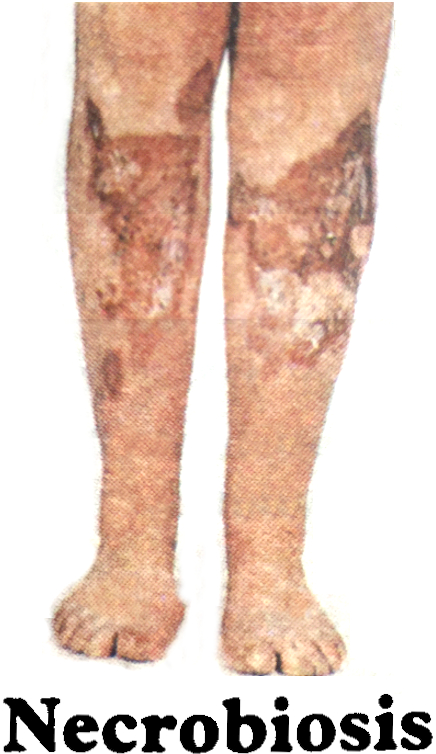
\includegraphics[scale=1.1]{images/072.jpg}\\
\textbf{\textit{Diabetic Dermopathy}}
\end{figure}

\textbf{Skin conditions caused by diabetes}

{
\small\addtolength{\tabcolsep}{-.9pt}
\begin{longtable}{|l|l|l|l|}
\hline
\multicolumn{1}{|c|}{\textbf{{Condition}}} & \multicolumn{1}{|c|}{\textbf{Appearance}} & \multicolumn{1}{|c|}{\textbf{Symptoms}} & \multicolumn{1}{|c|}{\textbf{Treatment}}\\
\hline
Diabetic &  Light brown, scaly, & None & This is a harm-\\
dermopathy & oval or round &  & less condition\\
 & spots usually seen &  & that needs no\\
 & on shin of legs &  & treatment\\
\hline
Necrobiosis & Starts as a dull, & Usually no & Protect your\\
Lipoidica & raised, red area. & symptoms. & legs and avoid\\
Diabeticorum & Later becomes & Sometimes & bumping into\\
This is a rare & a shiny scar with & itchy and & objects.If an\\
condition & a violet border. & painful. & ulcer develops\\
mostly & Usually seen over & Rarely  it & consult your\\
seen among & shins. & cracks. & physician for\\
women &  &  & treatment\\
\hline
Diabetic & Blisters appear & Usually none, & None in general.\\
blisters & over back of & except if they & They resolve on\\
 & fingers, hands, & rupture, in & their own in\\
 & toes and & which case & approximately\\
 & feet. Sometimes & there is pain & 3 weeks. If they\\
 & also seen over & and risk of & rupture, then\\
 & legs and & infection. & consult your\\
 & forearms. &  & doctor.\\
\hline
Eruptive & Yellow pea-like & Itch & Treat diabetes\\
Xanthoma- & bump surrounding &  & and high\\
tosis  & red halo found on & & cholesterol\\
 & back of hands, &  & which are the\\
 & feet, arms, legs \& &  & causes of this\\
 & buttocks. Usually &  & condition.\\
 & seen in type 1 &  & \\
 & diabetes, caused &  & \\
 & by high fat &  & \\
 & content in blood. &  & \\
\hline
Acanthosis & It is a sign of & None & Weight loss.\\
Nigricans & underlying &  & Screen these\\
 & insulin resistance, &  & patients for\\
 & and is mostly &  & diabetes, if not\\
 & seen in obese &  & already known.\\
 & people. Darkening &  & \\
 & of skin especially &  & \\
 & over nape of &  & \\
 & the neck, armpits &  & \\
 & and groin. Some- &  & \\
 & times over hands, &  & \\
 & elbows and knees. &  & \\
\hline
\end{longtable}
}\relax


\newpage
 
\setcounter{chapter}{17}
\renewcommand{\thechapter}{\arabic{chapter}B}
\chapter{Dental disease and diabetes}\label{chap18B}

This chapter is contributed by Dr. K.L.Sunil Tejaswi, Reader, Department of Endodontics and Conservative Dentistry, JSS Dental College, Mysore, Karnataka.

You may be surprised to know that there are more bacteria in your mouth than the entire human population on this planet! But it is\break reassuring to know that these bacteria peacefully co–exist with us and do not cause disease, except in rare circumstances. Unfortunately,\break diabetes is one such condition. Diabetics are more prone to oral infe\-ctions, specifically infections of the gums. These gum infections (called \textit{gingivitis\index{Gingivitis}}) are a culmination of some unique abnormalities caused by\break diabetes, and some irresponsible human behaviors.

\textit{“Gingiva”} is the latin word for gums. The gums form a tight seal around our teeth, and keep the teeth firmly in their sockets. If not for this tight seal, our teeth would move or get displaced out of their\break sockets when we bite into something hard or tough, like meat, sugarcane, raw mango, guava, etc.

Good dental hygiene is essential to keep our gums healthy. When we get lazy and neglect our gums, plaque builds up. Plaque is a sticky film or membrane that forms at the gum line, i.e. at the junction of the tooth and the gum. Plaque is composed of food, saliva, and bacteria.

The bacteria in the plaque infect the gums and cause a condition known as “gingivitis”. As a result of this, the gums become swollen, turn red, and bleed easily.

Having diabetes makes it easy for the bacteria to multiply and cause infections because of two reasons. The high blood sugar serves as a good food source for the bacteria. Secondly, the high blood sugar\break inhibits the white blood cells, which are responsible for fighting off infections.

If we ignore \textit{plaque\index{Plaque}} (despite it looking extremely distasteful to\break others and to yourself in the mirror!), then it hardens to form tartar. This is just like cement that hardens when left to dry. Unlike plaque, which forms at the gum line and is usually visible, tartar forms below the gum line. It accumulates between the gums and the teeth, and thus separates the two. Thus the tight seal between the gums and the teeth is lost. Bacteria enter this gap and cause infections here, which is called \textit{“periodontitis”\index{Periodontitis}}. These infections destroy the bone around the tooth. This bone forms the socket for the teeth, and when the socket is destroyed, the teeth become loose and fall out.

So now you know how diabetes affects our dental health. It is also important to remember that infections of the gums worsen diabetes control. Any infection in the body, will cause the blood sugar levels to spike, and this can even result in dangerous (and sometimes fatal) complications such as diabetic \textit{ketoacidosis (DKA)\index{Ketoacidosis}}.

\begin{figure}[h]
\vskip-.2cm
\centering
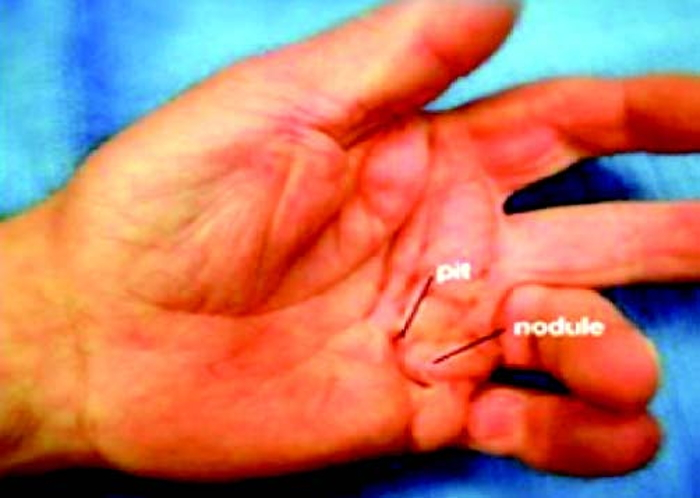
\includegraphics[scale=2.1]{images/073.jpg}
\vskip-.3cm
\end{figure}

\noindent\textbf{How can we prevent diabetes from affecting dental health?}

The answer to this question is very simple and basic. Our teeth need regular maintenance to keep them healthy. Regular maintenance includes the following:

\vspace{-\topsep}
\begin{enumerate}[•]
\itemsep=0pt
\item Brush your teeth at least twice daily, and preferably after each meal.
\item Use a brush with soft bristles (to avoid damaging the gums and\break enamel).
\item Floss gently at least once a day, and preferably after each meal.\break Brushing alone will not get rid of food particles stuck in between teeth.
\item Rinse your mouth after flossing.
\item If you wear dentures, remove them and wash them daily.
\item Visit your dentist at least twice a year to have your gums cleaned, and plaque and tartar removed.
\item Avoid caffeine and carbonated beverages (such as Coke, Pepsi, etc).
\item Do not smoke. Smokers are 20 times more likely to have gum disease.
\item Drink sips of plain water frequently throughout the day.
\end{enumerate}
\vspace{-\topsep}

\noindent\textbf{When should you seek immediate dental care from a dentist?}

Regular dental care described above is an excellent way of preve\-nting diabetes from damaging our dental health. But if you experience the following, you should seek immediate care from your dentist:

\vspace{-\topsep}
\begin{enumerate}[•]
\itemsep=0pt
\item If your gums bleed easily (for example when brushing, or biting into food). This may indicate the presence of gingivitis.
\item If your gums are red and swollen. This may be a sign of gingivitis.
\item If you experience tooth pain or gum pain.
\item If you notice pus around your teeth or gums. This may be a sign of periodontitis.
\item If you have persistent bad breath despite brushing and flossing\break regularly.
\end{enumerate}
\vspace{-\topsep}

\noindent\textbf{Fungal infections of oral cavity}

There is a higher risk of fungal (or yeast) infections of the oral\break cavity in diabetics. There are two reasons for this:

\vspace{-\topsep}
\begin{enumerate}[•]
\itemsep=0pt
\item High blood sugars offer a favorable environment for the growth of microbes.
\item High blood sugars inhibit the body’s immune cells (specifically the white blood cells), which are not able to fight off infections.
\end{enumerate}
\vspace{-\topsep}

Candida species are the most common type of fungus causing these infections. Candida infection is called thrush. A white film is seen covering the inner surface of the oral cavity. It causes difficulty in swallowing. It is easily treated with anti–fungal medications, but good blood sugar control is essential to prevent it from happening again.

\newpage

\renewcommand{\thechapter}{\arabic{chapter}}
\chapter{Musculoskeletal complications}\label{chap19}

\vspace{-\topsep}
\noindent{\textbf{Frozen shoulder or adhesive capsulitis}}\index{Frozen shoulder or Adhesive capsulitis}

Frozen shoulder or adhesive capsulitis is a disorder of the conne\-ctive tissue that limits the normal range of movement of the\break shoulder. It is a common condition seen in 10 to 20\% of all diabetics worldwide. A recent study from India found that 18\% of diabetics had frozen shoulder.$^{\text{\cite{chap19–key01}}}$$^,$$^{\text{\cite{chap19–key02}}}$$^,$$^{\text{\cite{chap19–key03}}}$

It is considered to be result of inflammation in and around the joints, as a result of long–term high blood glucose levels. This leads to thicke\-ning of connective tissue.

Other risk factors for this condition include older age, immobility of the shoulder joint for reasons such as recent stroke, recent surgery requiring bed rest, etc.

\noindent The condition develops slowly over time in three stages:

\vspace{-\topsep}
\begin{enumerate}
\itemsep=0pt
\item \textbf{Painful stage:} There is pain with any movement in the shoulder joint. In some patients, the pain may be worse at night.
\item \textbf{Frozen stage:} Pain decreases, but the joint becomes stiff, and the patient is unable to move the joint much.
\item \textbf{Thawing stage:} There is no more pain, and the movement also starts to improve.
\end{enumerate}
\vspace{-\topsep}

\noindent However in some cases, there may be permanent disability.

\noindent\textbf{Treatment}

\noindent Depending on the stage of the disease, the following interventions can help:

\begin{enumerate}[i.]
\itemsep=0pt
\item Applying heat or cold compress to the shoulder to relieve the pain.
\item Painkillers during the painful period only.
\item Continuing to move the joint as much as possible at home.
\item Physical therapy to help restore normal movements in the joint. A physiotherapist can help with these exercises.
\item If there is no improvement in 1–2 years, then steroid injection into the shoulder joint, or surgery to remove the scar tissue may be needed.
\end{enumerate}
\vspace{-\topsep}

\noindent\textbf{Prevention}

This condition often occurs when patients are not using the\break shoulder joint. This usually happens when someone is recovering from a recent surgery, stroke etc. It is important to try to move the shoulder joints as much as possible to prevent this condition.

\vskip 4pt
\noindent{\textbf{Dupuytren’s contracture\index{Dupuytren’s contracture}}}
\vskip 4pt

This is a deformity of the hand. It is a result of a thickening of the connective tissue underneath the wrist or palm of the hand.  
\begin{wrapfigure}{l}{4.9cm}
\centering
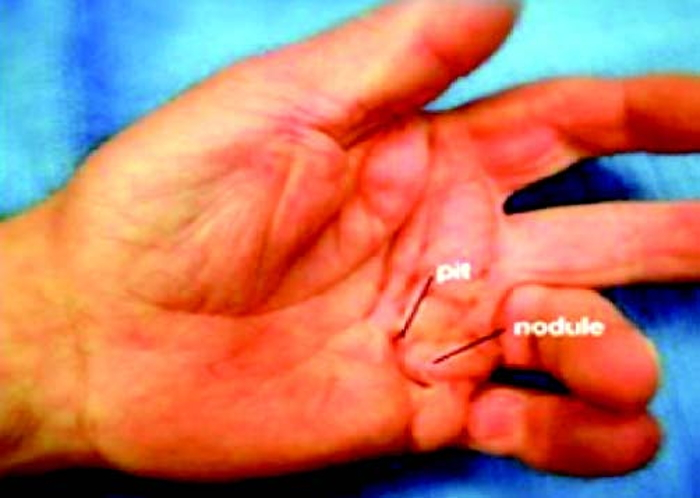
\includegraphics[scale=1]{images/074.jpg}
\vskip-.2cm
\end{wrapfigure}
This causes the fingers to be pulled into a bent position. Patients are\break unable to straighten their finger. Usually the ring finger and the\break little finger are affected. As a result even simple everyday activities such as holding a phone, driving, eating, etc become a struggle. According to some research, as many as 50\% of\break diabetics can suffer from this complication.$^{\text{\cite{chap19–key04}}}$

\vskip 5pt
\noindent\textbf{Treatment includes}
\vskip 2pt

\vspace{-\topsep}
\begin{enumerate}[•]
\itemsep=0pt
\item Pain medications as needed for pain relief.
\item Physical therapy to improve movement of the fingers.
\item Surgery to relieve the tightening of the connective tissue underneath the wrist and hand.
\end{enumerate}
\vspace{-\topsep}

\noindent{\textbf{Stiff Hand Syndrome or Diabetic Hand Syndrome}}

\begin{wrapfigure}{l}{4.5cm}
\vskip-.3cm
\centering
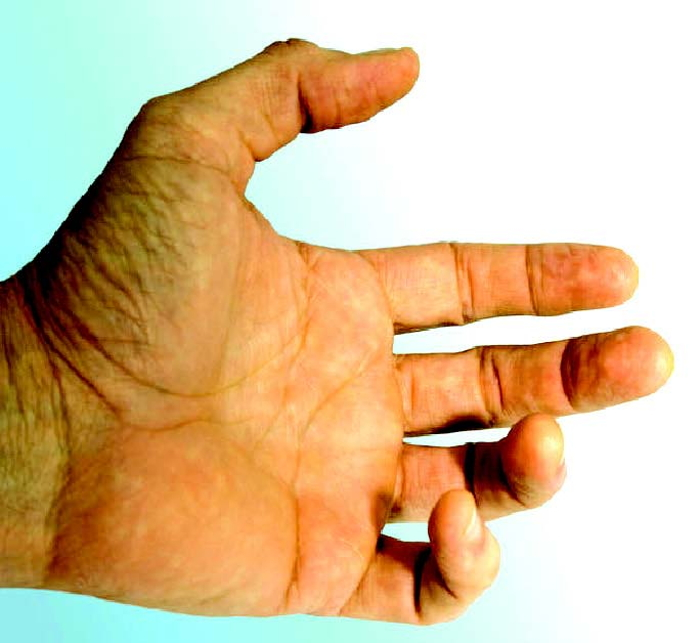
\includegraphics[scale=.9]{images/075.jpg}
\vskip-.3cm
\end{wrapfigure}

This can be seen in up to 35\% of diabetics and is thought to be a result of poorly controlled disease. The skin on the hands becomes thick, waxy and tight. When these patients are asked to bring their hands together, they are\break unable to do so, and form what is known as the “prayer hand”. This con\-dition causes an inability to move the fingers properly, and can severely limit even simple tasks like holding a glass, writing, etc. Physiotherapy and good blood sugar control can slow down the disease.

\vspace{-\topsep}
\begin{thebibliography}{99}
\itemsep=0pt
\bibitem{chap19–key01} Arkilla P, Kantola IM, Viidari JS, \& Ronnemaa T. Shoulder\break Capsulitis in type I and II diabetic patients: Association with dia\-betic complications and related diseases. Ann Rheum Dis. 1996; 55: 907–14.
\bibitem{chap19–key02} Pal B, Anderson J, Dick WC, \& Griffiths ID. Limitation of joint\break mobility and shoulder capsulitis in insulin– and non–insulin\break dependent diabetes mellitus. Br J Rheumatol. 1986; 25: 147–51.
\bibitem{chap19–key03} Ray S, Datta AK, Sinha Mahapatra R, Ray I, et al. Prevalence of rheumatic conditions in patients with diabetes mellitus in a\break tertiary care hospital. J Indian Med Assoc. 2011; 109 (2): 74–8.
\bibitem{chap19–key04} Noble J, Heathcote JG, \& Cohen H. Diabetes mellitus in the\break aetiology of Dupuytren’s disease. J Bone Joint Surg Br. 1984;\break 66 (3): 322–5.
\end{thebibliography}


\chapter{Diabetic gastroparesis}\index{Diabetic gastroparesis}\label{chap20}

Everday during our daily commute in the metros, we curse traffic jams, an unwanted evil of economic prosperity. But did you know that diabetes could cause traffic jam in your stomach! Yes, diabetic gastroparesis is nothing but a traffic jam inside the stomach. Normally it takes liquids like water, tea, etc about two hours to pass through the stomach. Solid food needs about four hours to move from the stomach into the small intestine.

The human stomach is like a pouch or a bag. The wall of this pouch is made of muscles.  
\begin{figure}[h]
\vskip-.4cm
\centering
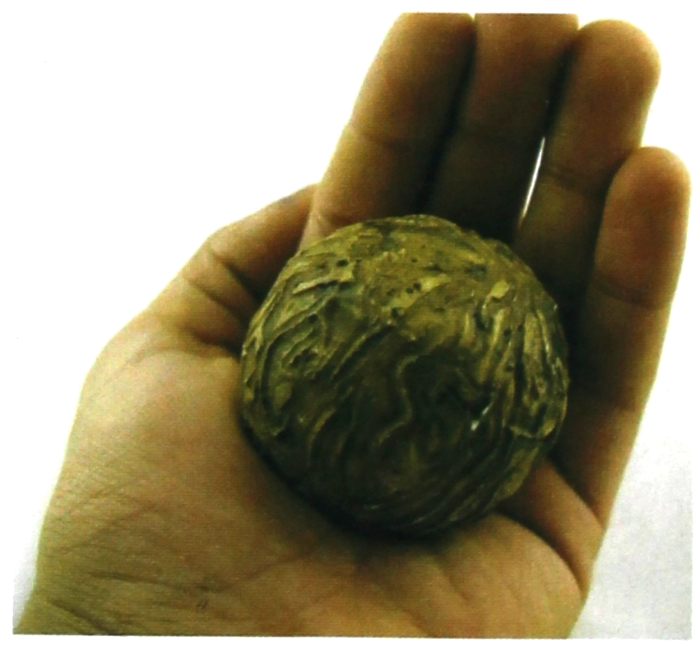
\includegraphics[scale=1.5]{images/076.jpg}\\
\textbf{\textit{Picture showing the roll of Vagus nerve\\ to control the movements of the stomach}}
\vskip-.5cm
\end{figure}
Just as muscles help us move our arms and legs, the stomach muscles help move food forward into the intestines. All muscles in the human body are controlled by the nervous system. The stomach muscles are under the control of a special nerve called the vagus nerve. In Latin vagus means to ‘wander’. As a matter of fact, the vagus nerve wanders through many parts of the human body, and controls actions of the heart, lungs, blood vessels, and stomach.

When diabetes is not well controlled, the high blood sugars\break affect the various nerves in our body. This is known as \textit{neuropathy}.\break Neuropathy will eventually affect the vagus nerve too. The excess\break blood glucose becomes toxic for the nerve. Slowly the vagus nerve starts to loose control over the stomach muscles. The plight of the stomach muscles is like that of an army without a leader, which has\break no idea about which direction to march in! Thus the muscles fail to\break propel food forward, and food gets stuck in the stomach for long\break periods of time. It is as if the stomach muscles are paralysed, and hence the name ‘gastroparesis’ or ‘paralysis of the stomach’.

\noindent\textbf{What are the symptoms of gastroparesis?}
\begin{enumerate}[•]
\itemsep=0pt
\item Stomach feels full even with small amounts of food
\item Bloating of the abdomen
\item Stomach pain
\item Feeling of wanting to vomit (nausea)
\item Vomiting undigested food
\item Heartburn or acid reflux
\item Lack of appetite.
\end{enumerate}

\noindent\textbf{What are the complications of \textit{gastroparesis?\index{Gastroparesis}}}

\begin{enumerate}[\ding{118}] 
\itemsep=0pt
\item It severely affects glucose control. Blood sugar levels swing wildly between lows and highs.

When the patient is unable to tolerate food, the body is unable to get sufficient nutrition. Blood sugar levels can plummet or drop steeply, and dangerous hypoglycemia may result.

Blood sugar can also dip if the patient takes medications or insulin without eating food.

On the other hand when food that has been delayed in the stomach for a long time finally enters the intestine and gets absorbed, the blood sugar level suddenly shoots up!

Blood sugar may also be high due to the patient not being able\break to take his medications due to the stomach pain, nausea etc. in\break addition, even if he takes medicines, he may vomit them out!

Due to these various reasons there is poor glucose control, and poor diabetes control, which only worsens the complications of diabetes, including gastroparesis. Thus the patient is thrown into a vicious cycle!
\item Patient may be unable to take other medications for blood pressure control, heart disease, etc.
\item \textit{Bezoar formation\index{Bezoar formation}}. When food is stuck inside the stomach for prolonged periods, the food can become hard and turn into a solid mass known as bezoar.
\end{enumerate}

\begin{wrapfigure}{r}{4.9cm}
\vskip -.4cm
\centering
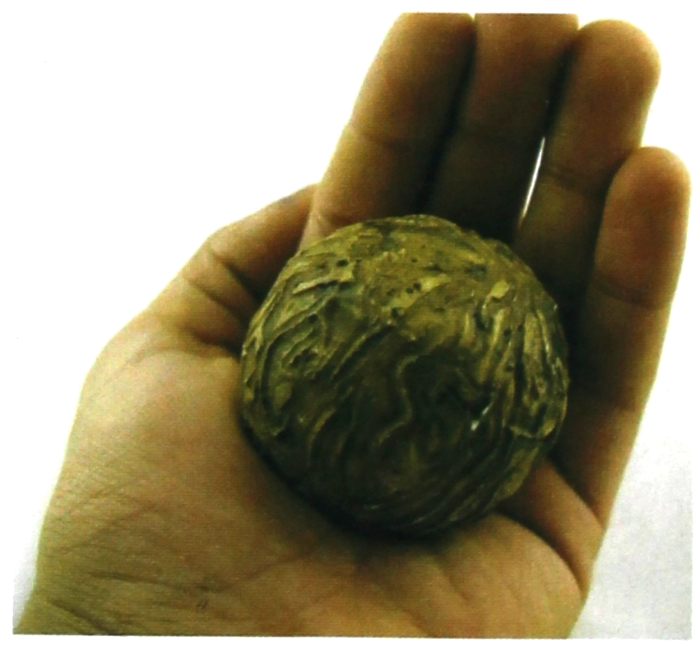
\includegraphics[scale=1.2]{images/077.jpg}\\
\textbf{\textit{Bezoar removed from the stomach}}
\end{wrapfigure}

\noindent\textbf{How is gastroparesis diagnosed?}

Simple tests are now available that can accurately estimate how well the stomach is emptying, and how well the muscles of the stomach are functio\-ning. Some of these tests are:
\begin{enumerate}[•]
\itemsep=0pt
\item Radioisotope gastric emptying study
\item Gastric manometry
\item Barium x–ray.
\end{enumerate}

\clearpage

\noindent\textbf{How is diabetic gastroparesis treated?}

Managing this condition requires efforts on part of both the patient and physician.

There are 2 components to treatment — strict blood sugar control and dietary changes.

Controlling blood sugar is very challenging because one cannot predict how much food the patient will tolerate, and if the person will be able to eat any food at all without vomiting it completely!

\noindent A few practical tips would be to:

\vspace{-\topsep}
\begin{enumerate}[•]
\itemsep=0pt
\item take insulin after eating.
\item check blood sugar levels more frequently and adjust insulin dose as needed.
\end{enumerate}
\vspace{-\topsep}

You should not however, make changes to your medications\break without first consulting your treating physician.

Regarding food, there are certain foods that should be avoided in gastroparesis, because they can worsen the symptoms. These include:

\vspace{-\topsep}
\begin{enumerate}[•]
\itemsep=0pt
\item High fiber foods—these foods are difficult to digest for patients with gastroparesis.
\item Fatty foods—they take a long time to digest in general, and hence are not well suited for diabetic gastroparesis.
\item Other foods such as coffee, tea, colas, etc.
\end{enumerate}
\vspace{-\topsep}

\noindent\textbf{In addition, some other measures that are useful include:}

\vspace{-\topsep}
\begin{enumerate}[•]
\itemsep=0pt
\item Eating small quantity meals more frequently, instead of large meals at one time.
\item Consuming more liquids than solids, since liquids are more easily\break digested than solids.
\end{enumerate}
\vspace{-\topsep}


\chapter{Sexual dysfunction in diabetes}\label{chap21}

\noindent{\textbf{Male sexual dysfunction}}

Age can humble even the greatest of men by striking where it\break matters the most! Impotence is probably the most embarrassing\break change that accompanies age. \textcolor{red}{\textit{A man with diabetes is three times more likely to suffer from impotence. To make matters worse, impotence affects\break diabetic men 10–15 years earlier than usual. In fact, between 35–70\% of all diabetic men suffer from impotence.}}

\noindent\textbf{What is impotence or \textit{erectile dysfunction?\index{Erectile dysfunction}}}

It is the inability to obtain an erection, or maintain an erection long enough. Libido or sexual desire is intact, which makes impotence even more frustrating.

\noindent\textbf{What is the cause of impotence or erectile dysfunction in dia\-betics?}

In order to understand what goes wrong, it is important to try to understand what is the mechanism of an erection.

\noindent There are 2 main components to an erection:

\vspace{-\topsep}
\begin{enumerate}
\itemsep=0pt
\item \textbf{Nervous system:} Two kinds of neural impulses can trigger an erection:
\begin{enumerate}[a)]
\itemsep=0pt
\item Central stimulus– a desire to have sex arising in the brain
\item Local stimulus– tactile (touch) stimulation of the penis

Either of these stimuli causes an electrical current to flow through the nerves that connect the nervous system and the penis. These nerves will stimulate the blood vessels of the\break penis, and cause an increase in blood flow into the penis. In addition, due to some special changes the blood cannot flow out of the penis. Hence for a brief period of time, there is an excess amount of blood trapped inside the penis, which causes the penis to become enlarged and rigid. This is no\break different than a balloon filled with water.
\end{enumerate}
\item \textbf{Blood supply:} The penis is supplied by very tiny blood vessels. Inside the penis, there are 2 chambers called corpora cavernosa. These chambers are usually collapsed. But when blood flow to the penis increases, these chambers fill up with blood and\break expand just like 2 balloons filled with water. When these\break chambers expand with arterial blood, they squeeze the veins of the penis and cause them to collapse. As you know, veins are\break responsible for carrying blood back from all organs of the body to the heart. With the veins compressed, the blood gets stuck\break inside the 2 chambers of the penis, and hence an erection is\break maintained for some time.

Now that you know the mechanism of an erection, it is easier to understand how diabetes affects this, resulting in impotence.
\begin{enumerate}[i.]
\itemsep=0pt
 \item \textbf{Autonomic neuropathy:}

The autonomic nervous system is in charge of mobilizing the small blood vessels that supply the penis. It is only when these small blood vessels dilate and allow more blood flow through them into the chambers of the penis (corpora\break cavernosa), that an erection becomes possible. But diabetes affects the autonomic nervous system. Thus, even though a desire arises in our mind, the nerves are unable to translate this desire into an erection.

 \item \textbf{\textit{Vasculopathy\index{Vasculopathy}:}}

The 2nd essential ingredient of an erection is increased\break blood flow through the delicate blood vessels of the penis. The blood vessels have to dilate and pump more blood into the penis, and basically inflate the penis like a water–filled balloon. But in diabetes, the walls of these small arteries\break become stiff and their diameters become smaller. Hence they are unable to stretch and pump more blood into the penis, and thus, an erection never takes off.
\end{enumerate}
\end{enumerate}
\vspace{-\topsep}

\noindent\textbf{How can diabetes induced impotence be treated?}

Thanks to medical innovation, the flagging male pride can be\break restored in those rendered impotent by diabetes.

The pill ‘Viagra’ has now become a well–known medication. Viagra causes the muscles in the walls of the small blood vessels supplying the penis to relax or stretch out. This causes the vessels to dilate and allow more blood to flow through them into the penis.

Several other medications have also been invented that work\break similar to ‘Viagra’, and they include– ‘tadalafil’ and ‘vardenafil’.

\noindent\textbf{Precaution while using ‘Viagra’ or similar drugs}

The mechanism of action of Viagra involves relaxation of smooth muscles in the walls of blood vessels that supply the penis. While it predominantly affects the blood vessels of the penis, to some extent it can cause the same effect in other blood vessels in the rest of the body too. As mentioned in previous chapters, in order for blood to flow back to the heart, the blood vessels have to push against gravity to move blood from the lower body into the heart. The blood vessels manage to do this by squeezing. This squeezing action is a result of contraction of the muscles in the walls of the blood vessels. But Viagra can prevent this muscle contraction. Blood pools in the lower extre\-mi\-ties, and there is less blood reaching the heart, consequently there is less blood being pumped out of the heart, and thus less blood reaching the brain.

This whole situation is compounded by the fact that many diabe\-tics are also taking medications for hypertension. The combination of Viagra and blood pressure medications can cause the blood pressure to drop to precipitous levels. This can be dangerous enough to cause the brain cells to be starved of oxygen and end up with a stroke and even death!

Hence it is very important to consult with your doctor before\break starting Viagra or similar drugs. Of course, men would naturally feel very awkward to initiate this discussion, let alone admit that they are unable to have erections. Hence it is important that the doctors also actively participate in this process and inquire about sexual difficulties in their diabetic patients.

\textbf{A final word of caution is that nitrates and ‘Viagra’ should never be mixed!} Nitrates are medications prescribed to treat chest pain in people with coronary heart disease. By nature these medicines cause low blood pressure. Mixing Viagra with nitrates can cause\break dangerously low blood pressure.

\noindent\textbf{Sexual dysfunction in women}

Discussing sexual health, that too among women in India is very taboo. But we know from studies conducted in other countries that diabetic women suffer sexual dysfunction. It has been seen that 35\% of type 1 diabetic women and 53.4\% of type 2 diabetic women suffer from sexual dysfunction.$^{\text{\cite{chap21–key01}}}$$^,$$^{\text{\cite{chap21–key02}}}$ While sexual dysfunction manifests as impotence (erectile dysfunction) among men, it assumes several forms among women, and includes:

\vspace{-\topsep}
\begin{enumerate}[•]
\itemsep=0pt
\item Decreased desire for sexual activity—usually from depression and side effects of medicines commonly used to treat associated hypertension
\item Uncomfortable or painful sexual intercourse—usually from dryness or lack of lubrication.
\item Decreased or absent pleasure from sexual activity—from nerve\break damage, lack of adequate genital lubrication, etc.
\end{enumerate}
\vspace{-\topsep}

\noindent The causes for these dysfunctions include:

\vspace{-\topsep}
\begin{enumerate}[•]
\itemsep=0pt
\item Autonomic neuropathy—this affects the nerves of the vaginal area; sexual desire in the brain is conveyed via nerves to the vagina,\break and sensations from the vagina are conveyed via nerves to the brain. Nerves stimulate the blood vessels of the genital area and increase blood flow to the area. The nerves also stimulate increased fluid\break secretion in the genital area that helps with lubrication. But in dia\-betes, all these functions are compromised.
\item Vasculopathy—this affects the blood vessels supplying the vaginal area; normally during sexual arousal there is an increase in blood flow to the genital areas.
\item High blood glucose levels dampen sexual desire.
\item High blood glucose levels cause frequent vaginal yeast infections, which makes it unpleasant and uncomfortable to engage in sexual activity.
\item Side effects of commonly used medications in diabetes such as anti–hypertensives (beta blockers, diuretics), and anti–depressants, can lead to decreased libido or desire to engage in sexual activity.
\item Poor self image among diabetic women who are obese or overweight causes low self–esteem and decreased sexual desire.
\end{enumerate}
\vspace{-\topsep}

\noindent\textbf{Remedies to these sexual problems among diabetic women}

Sexual health, particularly among women in India is an extremely sensitive subject. However, a normal sexual life is integral to a happy and satisfactory marriage and leads to overall well–being. Hence,\break women with diabetes should talk to their gynecologist about their\break concerns and questions. Controlling the blood sugar levels, lubricant creams for the genital area, avoiding medicines that decrease libido, physical exercise, maintaining a healthy weight, talking to a counselor, etc are some of the many interventions that can improve the sexual health of diabetic women.

\begin{thebibliography}{99}
\bibitem{chap21–key01} Enzlin P, Rosen R, Wiegel M, Brown J, et al. Sexual dysfunction in women with type 1 diabetes: long–term findings from the DCCT/EDIC study cohort. Diabetes Care. 2009; 32 (5): 780–5.
\bibitem{chap21–key02} Esposito K, Maiorino MI, Bellastella G, Giugliano F, et al. Determinants of female sexual dysfunction in type 2 diabetes. Int J Impot Res. 2010; 22 (3): 179–84.
\end{thebibliography}


